\documentclass{beamer}

\mode<presentation>
{

  \usetheme{Boadilla}
  \usecolortheme{whale}
  \setbeamercovered{transparent}
  
  \setbeamertemplate{footline}[frame number]{}
  \setbeamertemplate{navigation symbols}{}

}

\usepackage[english]{babel}
\usepackage[utf8]{inputenc}
\usepackage{times}
\usepackage[T1]{fontenc}

\usepackage{amsmath, amsthm, amssymb, amsfonts}
\usepackage{mathtools}

\usepackage{graphicx}


\usepackage{natbib}
\bibliographystyle{unsrtnat}

\usepackage{float}
\usepackage{bbm}
\usepackage{mathrsfs}

% ======== Alix notation =======
\def\th{\theta}
\def\eps{\epsilon}
\def\beq{\begin{equation}}
\def\eeq{\end{equation}}
\def\bdm{\begin{displaymath}}
\def\edm{\end{displaymath}}
\def\vsd{\vspace{0.1in}}
% ==============================

\usepackage{listings}




\title{Take Me Out to (Analyze) the Ballgame}
\subtitle{Visualization and Analysis Techniques for Big Spatial Data}
\author{Chris Comiskey} 
\institute{Oregon State University} 
\date{\today} 

% Delete this, if you do not want the table of contents to pop up at the beginning of each subsection:

\AtBeginSection[]
{
 \begin{frame}<beamer>{Outline}
   \tableofcontents[currentsection,currentsubsection]
 \end{frame}
}

\AtBeginSubsection[]
{
 \begin{frame}<beamer>{Outline}
   \tableofcontents[currentsection,currentsubsection]
 \end{frame}
}

\begin{document}

\begin{frame}
  \titlepage
\end{frame}

% \section{Introduction}
% 
% \begin{frame}{Baseball, Baseball, Baseball} % ==================
% \begin{columns}
% \column{0.5\textwidth}
% \begin{itemize}
% \item Chris, rookie year
% \end{itemize}
% 
%         \begin{figure}[H]
%       	\centering
%       	\includegraphics[scale=.65]{Images/CWC_Royals.pdf}
%       	% Images only work with: setwd("~/Desktop/ResearchRepo/Seminar")
%       	\end{figure}
% 
% \column{0.5\textwidth}
% \begin{itemize}
% \item Chris, Boston Red Sox
% \end{itemize}
%   \begin{figure}[H]
% 	\centering
% 	\includegraphics[scale=.3]{Images/RedSox.jpg}
% 	\end{figure}
% 
% \end{columns}
% \end{frame}
% 
% \begin{frame}{Contributions (Sections) Road map}{}
% \begin{enumerate}
% \addtolength{\itemsep}{0.5\baselineskip}
% \item Variable-resolution heat maps, and {\bf varyres}
% \item Interactive confidence intervals, and {\bf mapapp}
% \item Approaches to Big N Spatial Generalized Linear Mixed Models (SGLMMs) for baseball data \\
%   \begin{itemize}
%   \addtolength{\itemsep}{0.5\baselineskip}
%   \item Optimizing in Stan \citep{STANtheMan}
%   \item Predictive Process Models (PPMs) \citep{Banerjee2008}
%   \item Integrated Nested Laplace Approximations (INLA) \citep{Rue2009}
%   \end{itemize}
% \end{enumerate}
% 
% \end{frame}
% 
% \begin{frame}{Hitting Analytics, Then and Now} % ==================
% \begin{columns}
% \column{0.5\textwidth}
% \begin{itemize}
% \item $\text{``The Science of Hitting''}_{\text{1970}}$
% \end{itemize}
% 
%         \begin{figure}[H]
%       	\centering
%       	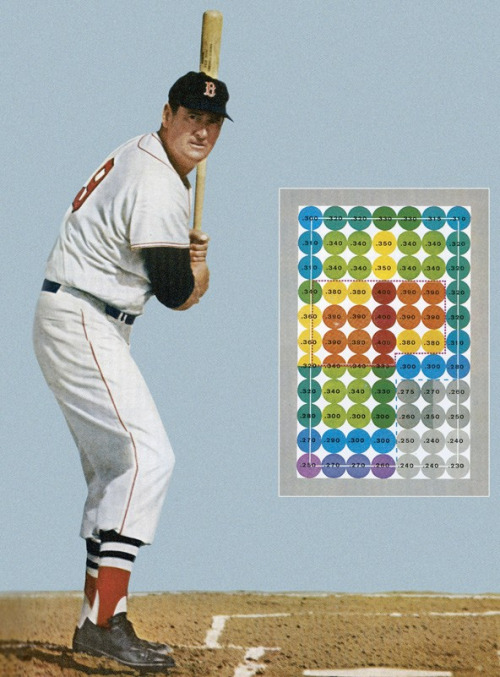
\includegraphics[scale=.22]{Images/Williams.jpg}
%       	% Images only work with: setwd("~/Desktop/ResearchRepo/Seminar")
%       	\end{figure}
%       
% \begin{itemize}
% \item Iconic breakthrough, hitter
% \item No data
% \end{itemize}
% 
% \column{0.5\textwidth}
% \begin{itemize}
% \item The Statistics of Hitting
% \end{itemize}
%   \begin{figure}[H]
% 	\centering
% 	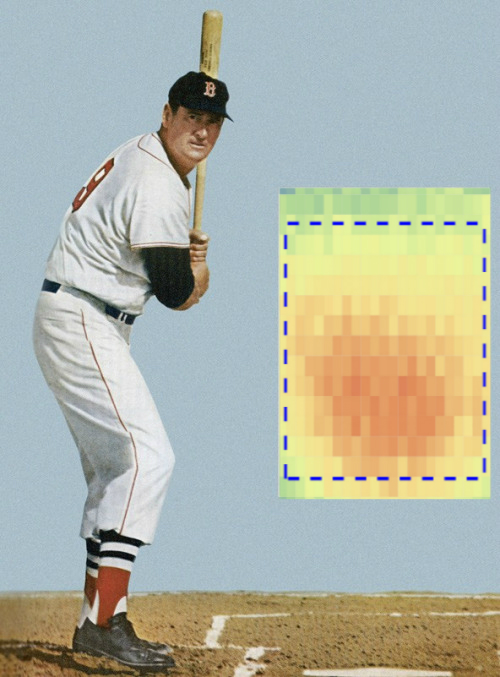
\includegraphics[scale=.22]{Images/WilliamsMother.jpg}
% 	\end{figure}
% \begin{itemize}
% \item PITCHf/x data, R, heat maps
% \item SGLMMs, Stan, PPMs, INLA
% \end{itemize}
% 
% \end{columns}
% \end{frame}
% 
% \section{Varible-Resolution Heat Maps}
% 
% \begin{frame}{Empirical Success Probability Heat Map} % =============
% \begin{columns}
% 
% \column{0.5\textwidth}
% 
%   \begin{figure}[H]
% 	\centering
% 	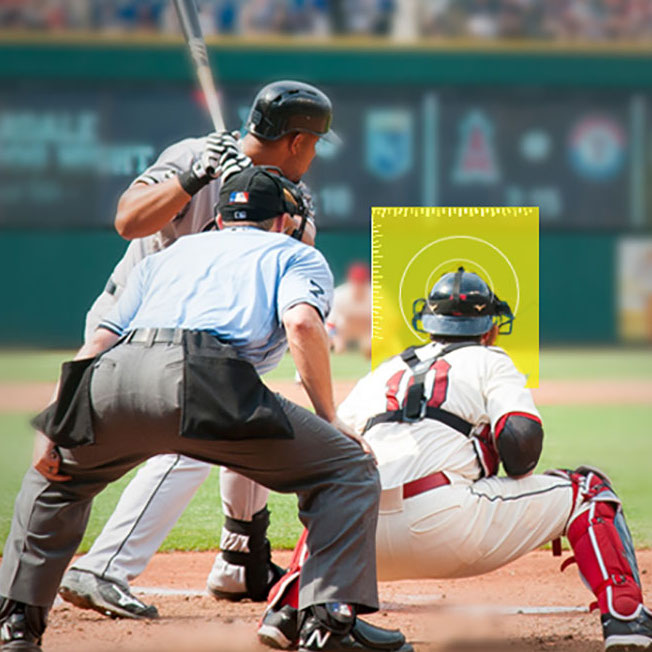
\includegraphics[scale=.26]{Images/StrikeZone3.jpg} 
% 	\end{figure}
% 
% \column{0.5\textwidth}
%   \begin{figure}[H]
% 	\centering
% 	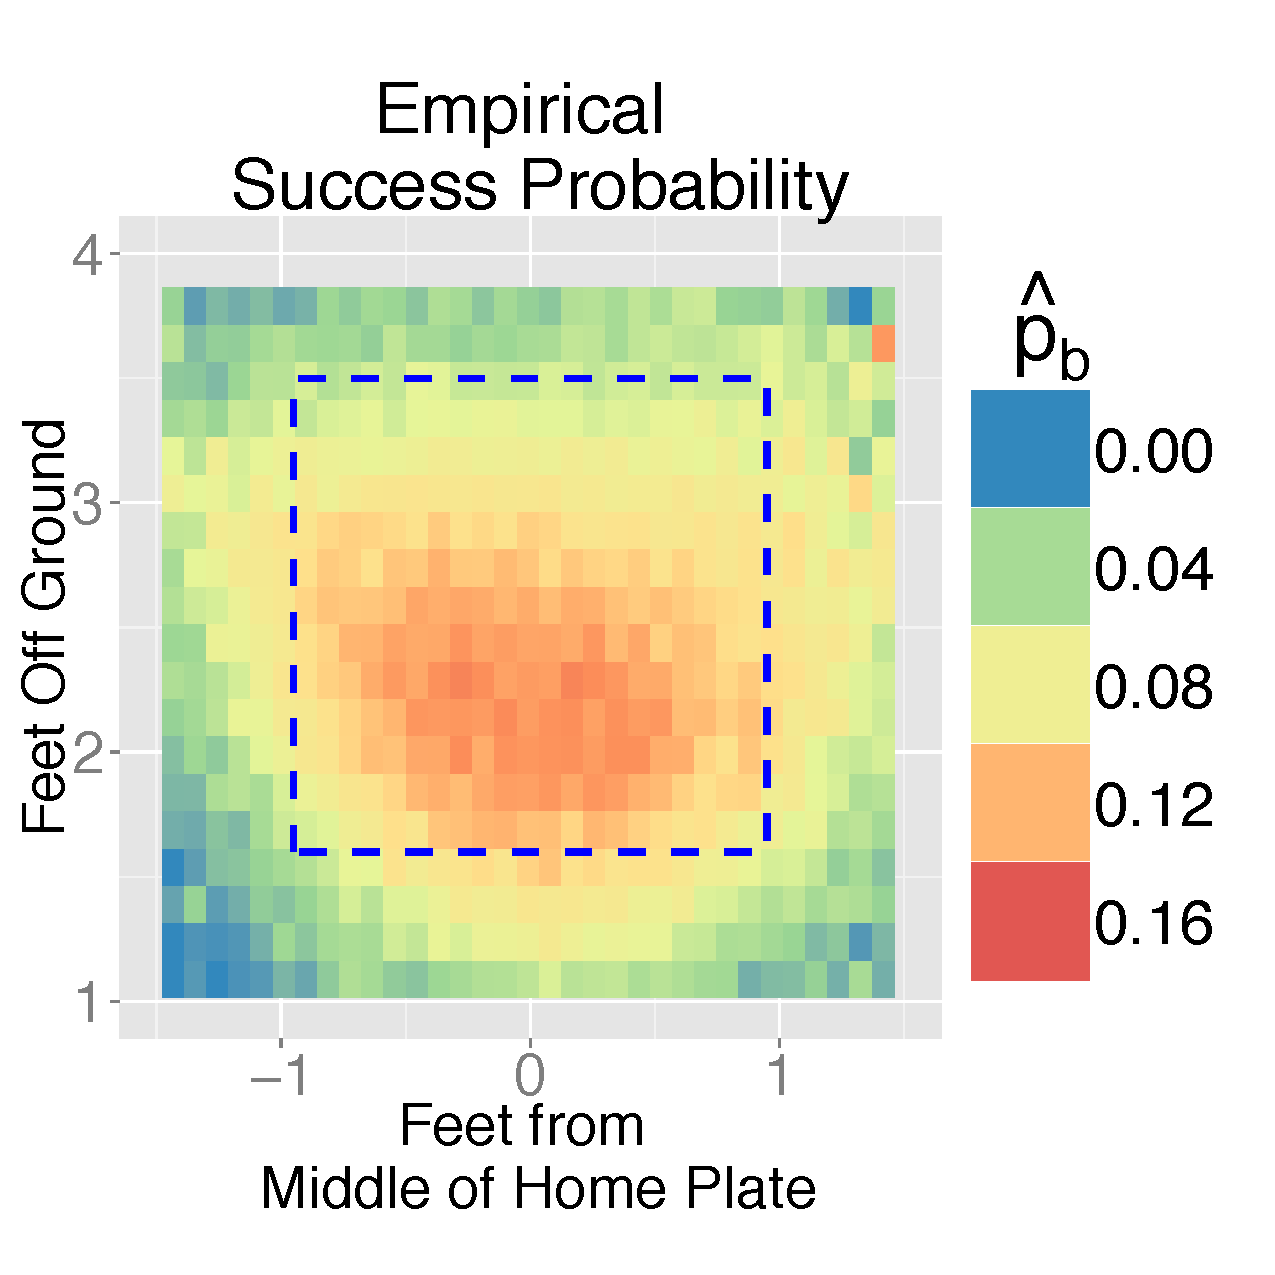
\includegraphics[scale=.07]{Images/Mothership.jpg} 
% 	\end{figure}
% 	
% \end{columns}
% \end{frame}
% 
% \begin{frame}{Empirical Success Probability Heat Map} % ====
% 
% \begin{itemize}
% \addtolength{\itemsep}{0.5\baselineskip}
% \item Swings: $i = 1,2,\ldots, N$; and $\pi_i = Pr(S_i = 1)$ where:
%     \bdm
%     S_i = \left\{\begin{array}{ll} 1; & \mbox{swing success} \\
%     					 0; & \mbox{swing failure} \\ \end{array} \right.
%     \edm
% 
% \item Pitch location $(x_i,y_i)$, grid boxes $G_1,G_2,\ldots,G_B$:
%     \bdm
%     N_b = \sum_{i=1}^N I_{(x_i,y_i) \in G_b}
%     \edm
% \item $\pi_b = \mbox{Pr(Swing success in }G_b)$, estimate with:
%     \bdm
%      p_b = \frac{1}{N_b} \sum_{i=1}^N S_i I_{(x_i,y_i) \in G_b}
%     \edm
% for $b = 1,2,\ldots,B$.
% \end{itemize}
% \end{frame}
% 
% \begin{frame}{Heat Map Resolution, Jhonny Peralta}{Compare Resolutions}
%   \begin{figure}[H]
% 	\centering
% 	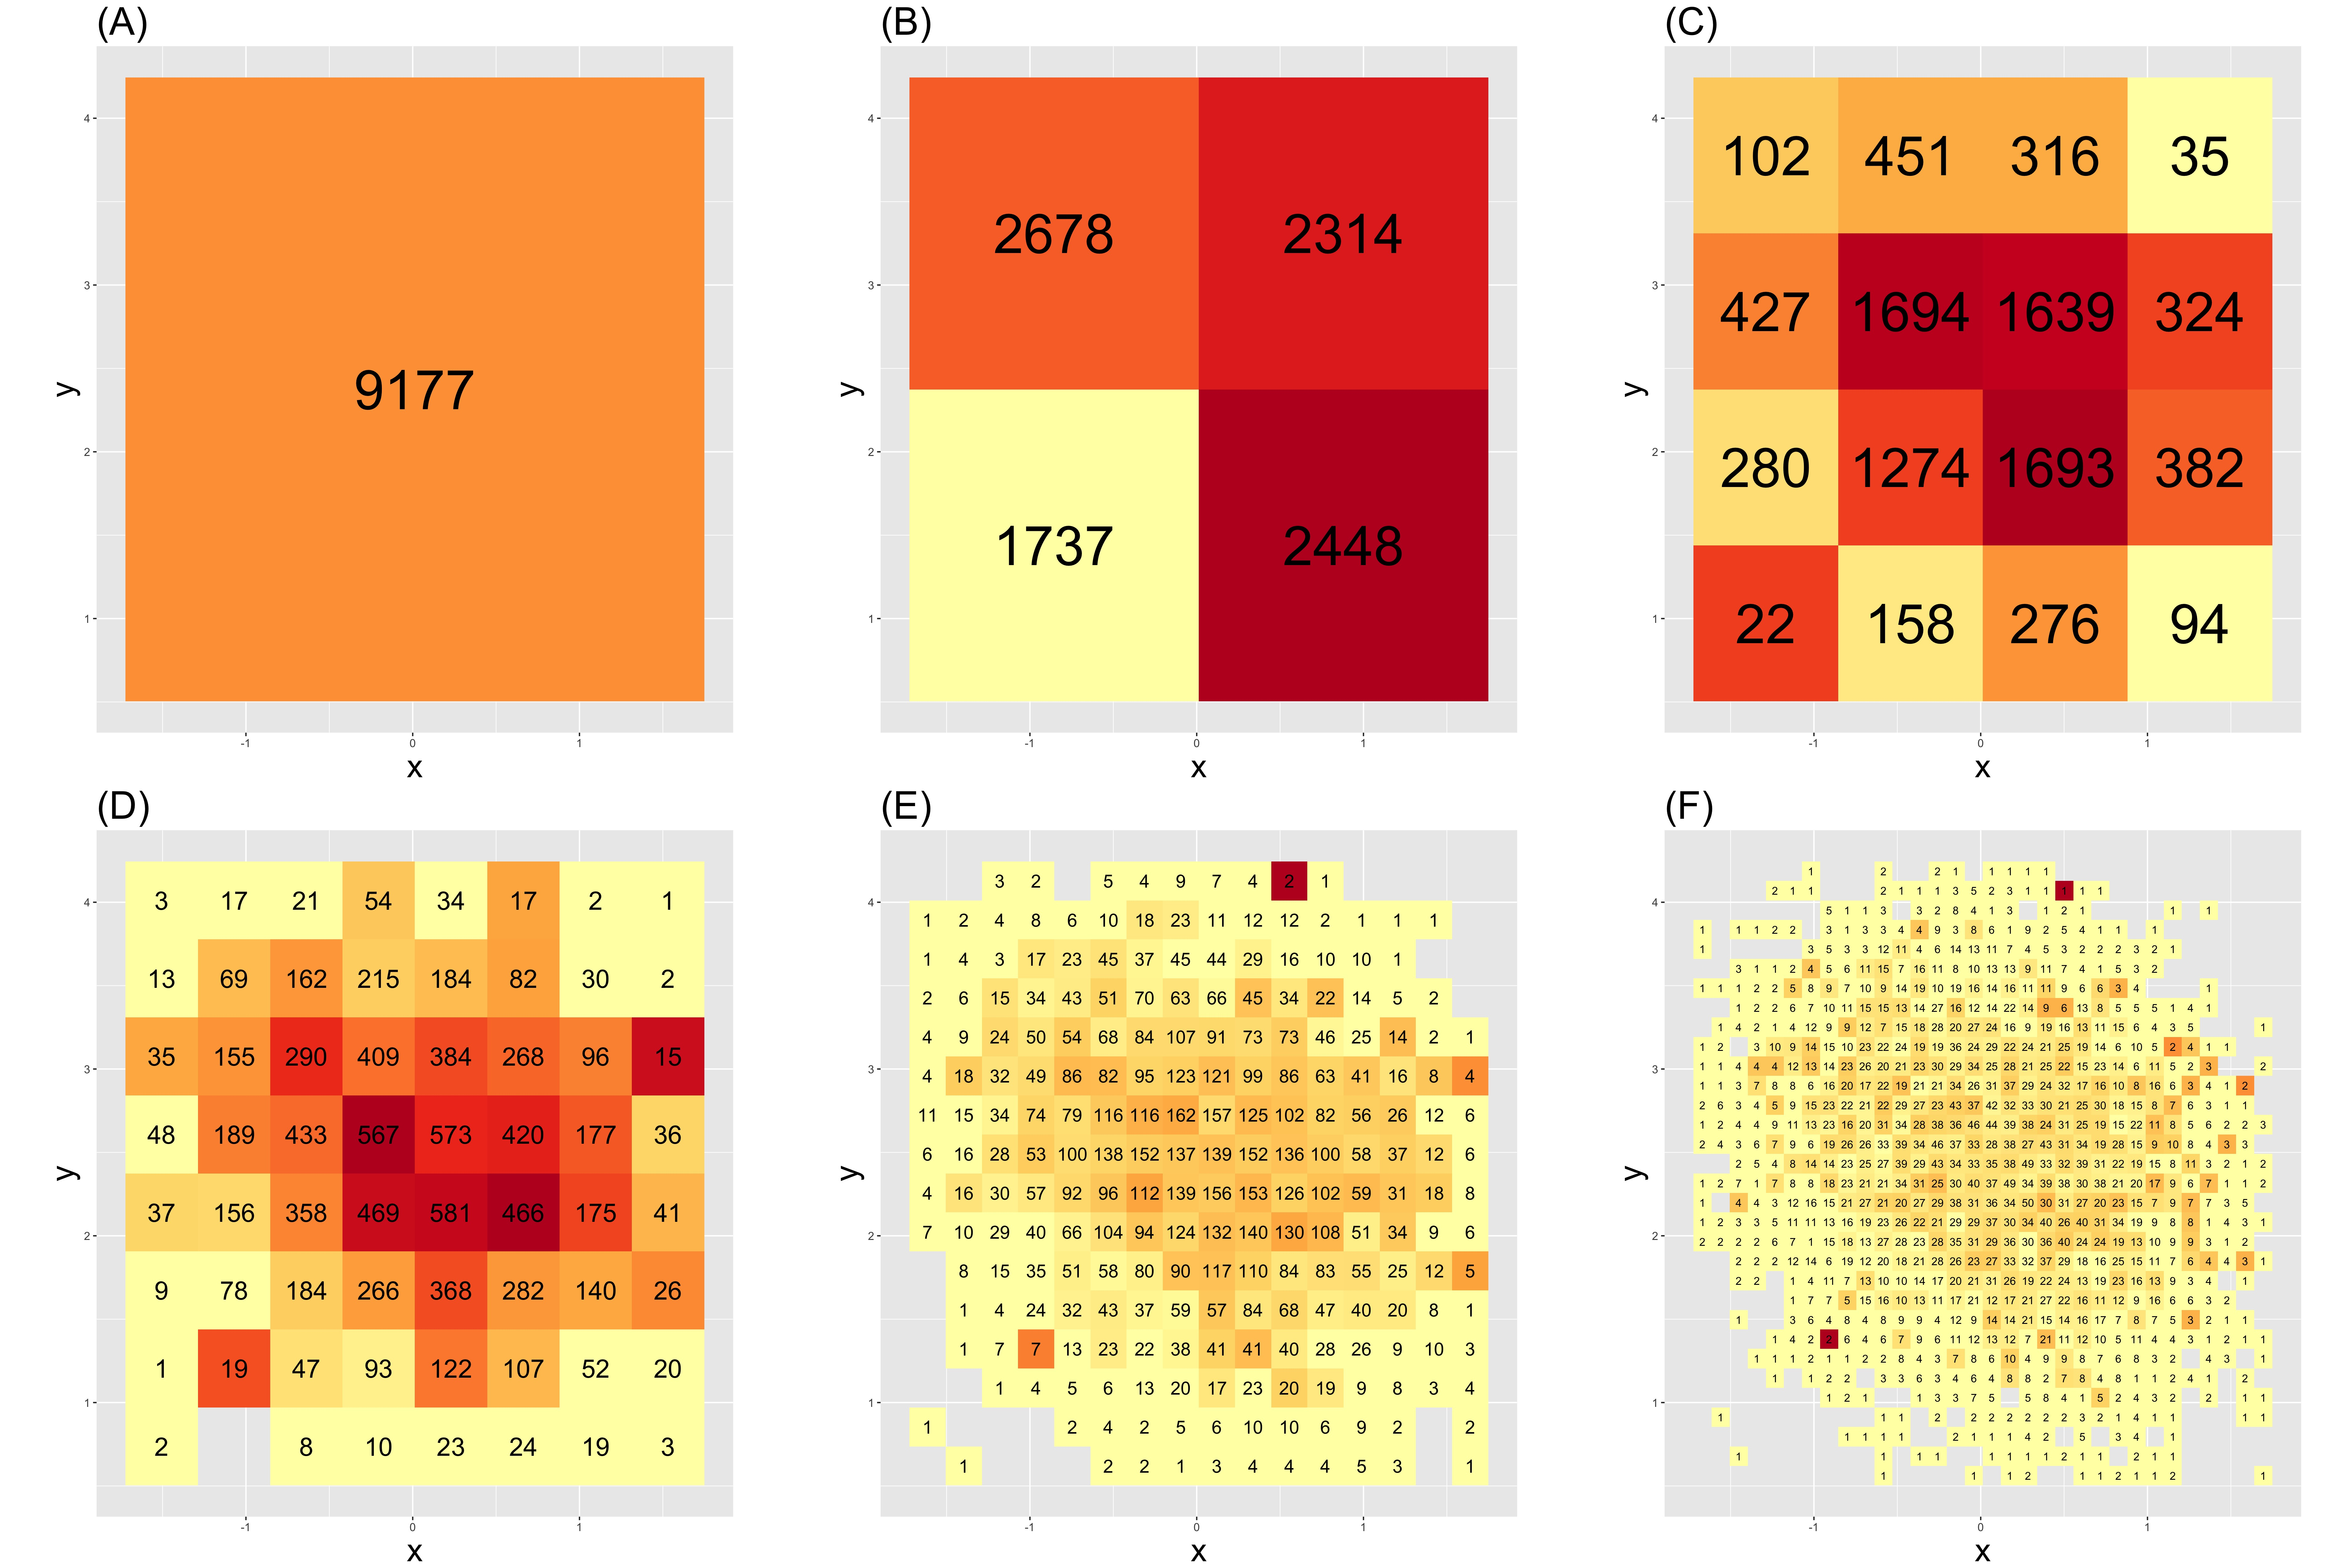
\includegraphics[scale=.0425]{Images/Chapter_VarRes.jpg}
% 	\end{figure}
% \end{frame}
% 
% \begin{frame}{Heat Map Resolution, Jhonny Peralta}{Combine Resolutions}
%   \begin{figure}[H]
% 	\centering
% 	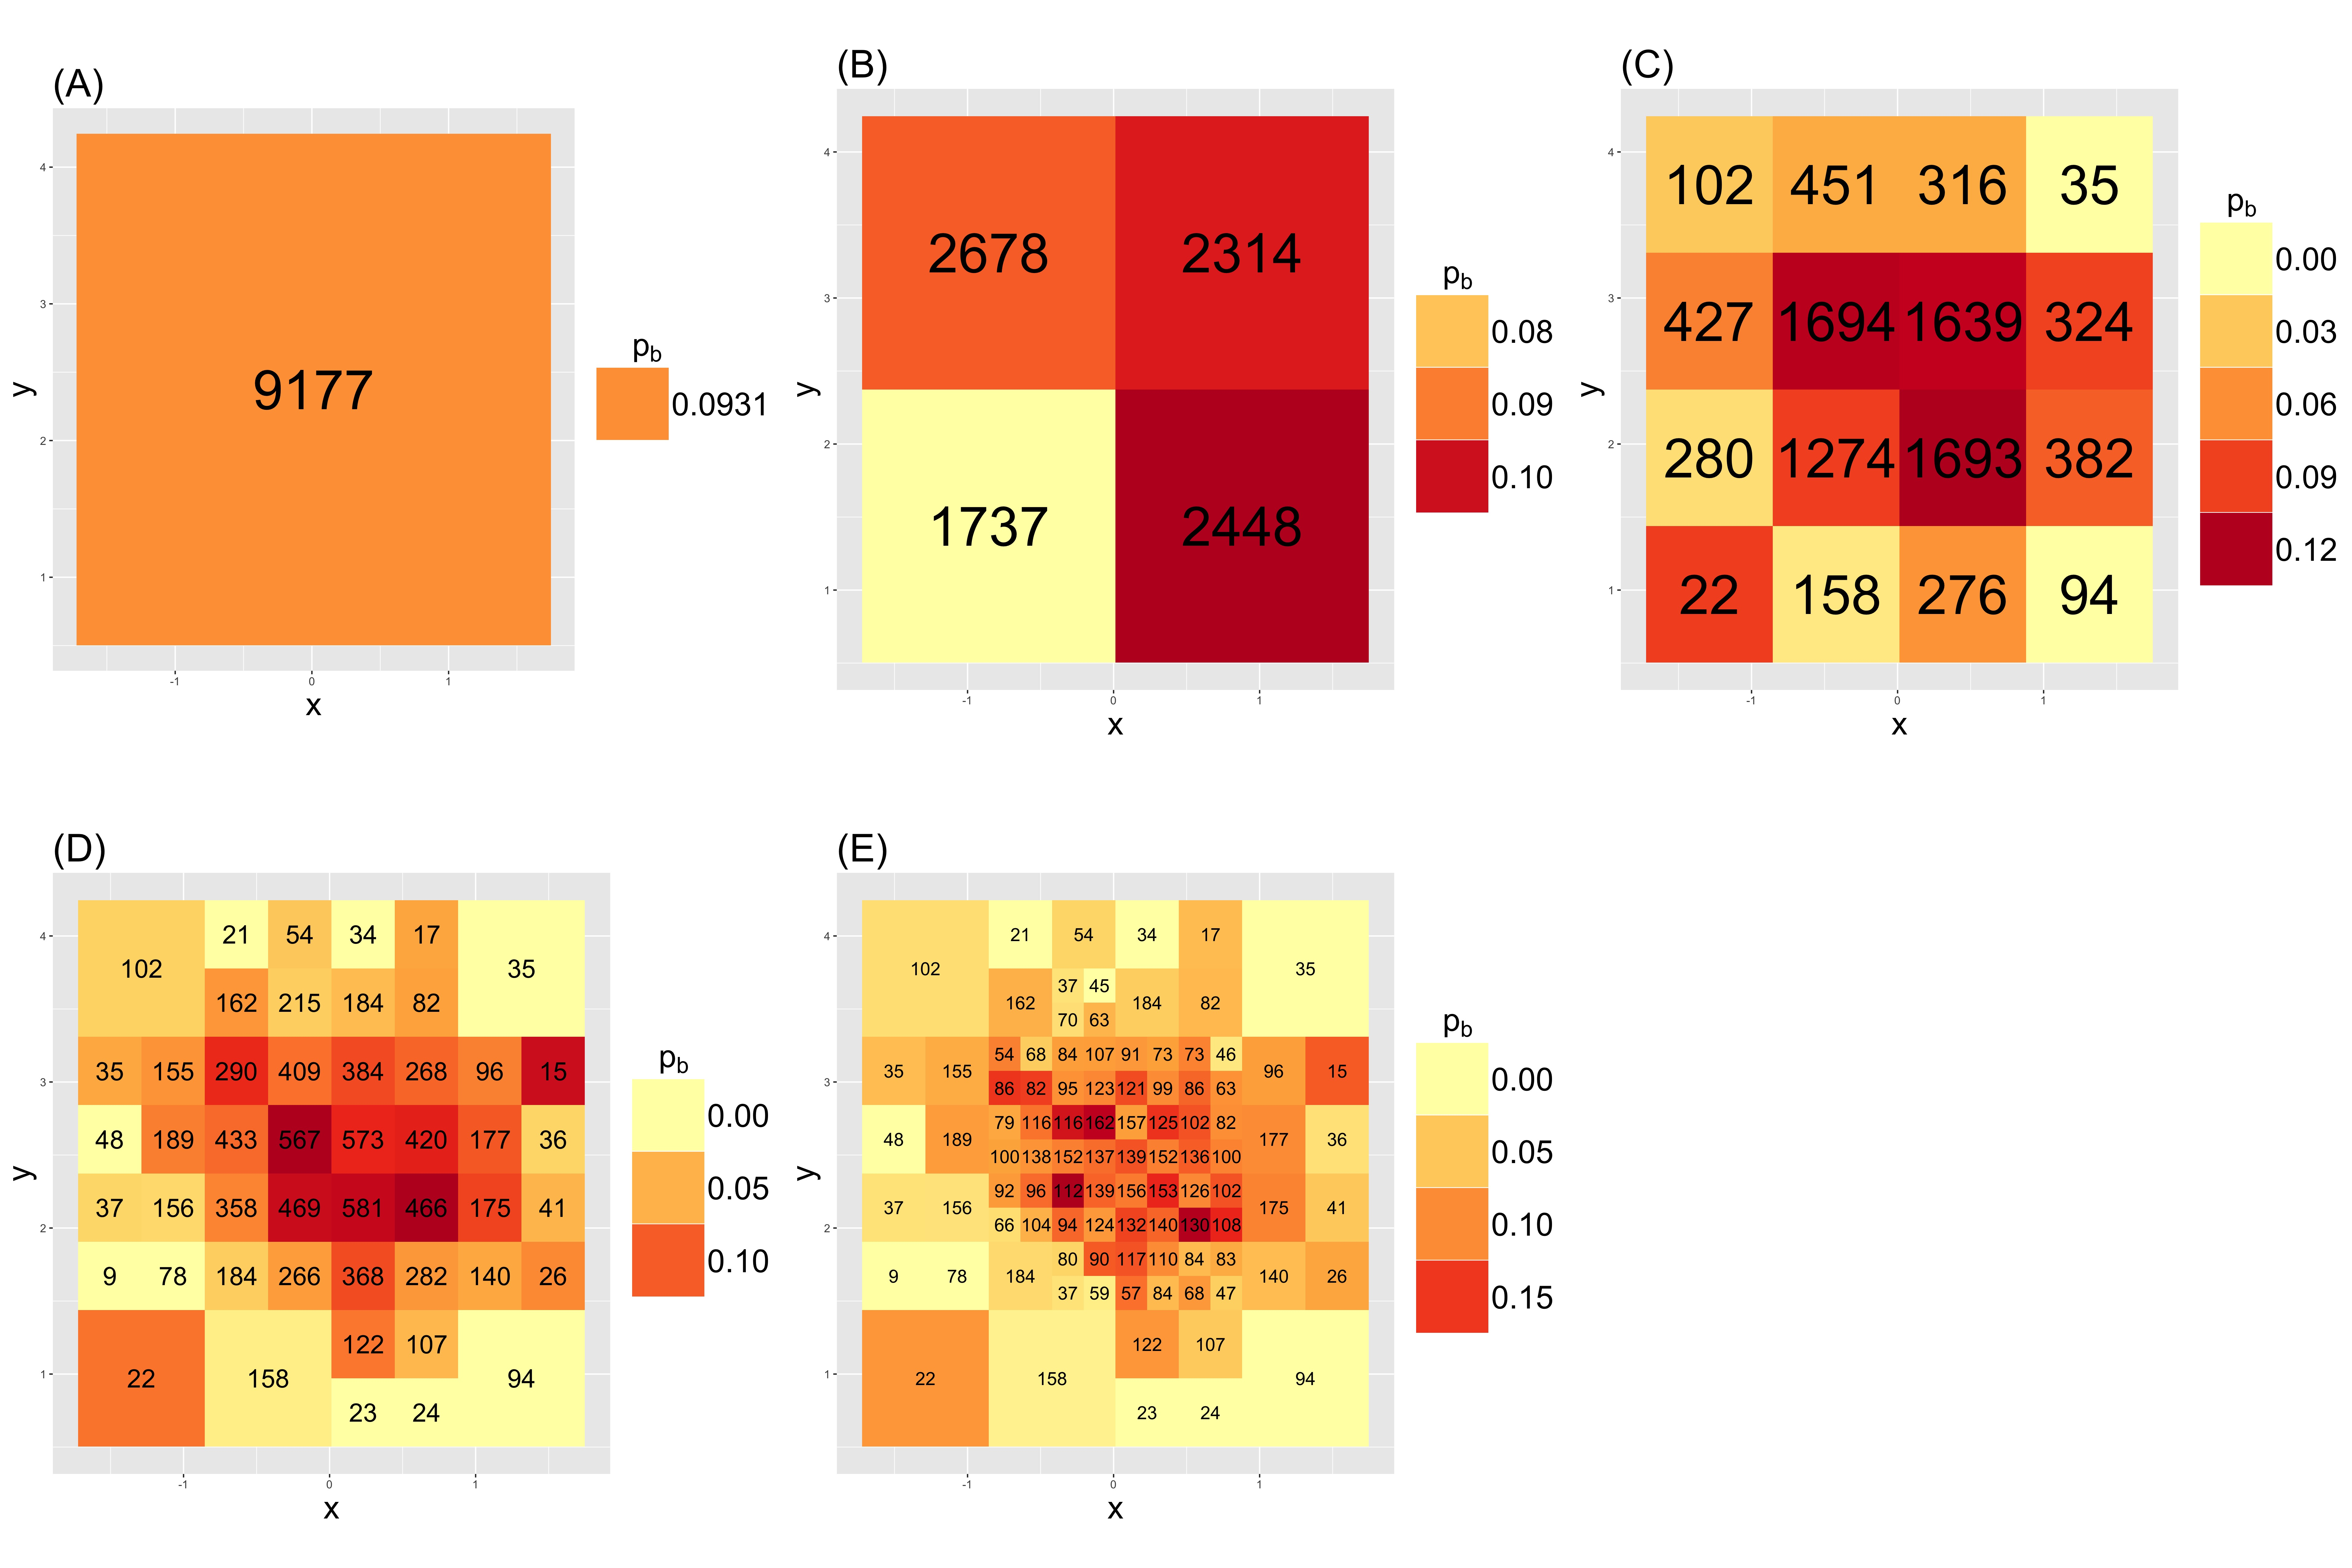
\includegraphics[scale=.0425]{Images/6_200.jpg}
% 	\end{figure}
% \end{frame}
% 
% \begin{frame}{Best of Both (Spatial) Worlds}{}
% \begin{itemize}
% \addtolength{\itemsep}{0.5\baselineskip}
% \item Location specific resolution, rather than one global resolution
% \item Stopping rule $\iff$ {\bf sample size}* threshold
% \item Local resolution conveys data density
%   \begin{itemize}
%   \addtolength{\itemsep}{0.5\baselineskip}
%   \item Big box $\iff$ low density
%   \item Bigger box, bigger variance*
%   \end{itemize}
% \item Choose subdivision algorithm
% \end{itemize}
% \end{frame}
% 
% \begin{frame}[fragile]{Variable-Resolution Algorithm}{Pseudo-code}
% * Keep track of three containers: History, Current, Iteration
% \begin{verbatim}
% function(dataset, 
%          fun = mean, # function to apply to box data
%          cutoff,     # stopping rule threshold
%          max ){      # maximum number of iterations
%          
% HISTORY_CONTAINER # store iterative results
% 
% CURRENT_CONTAINER: box centers, statistic, 
%   box observations, box heights/widths, 
%   box vert/horiz, upper/lower bounds
% 
% Add CURRENT_CONTAINER to HISTORY_CONTAINER
% \end{verbatim}
% \end{frame}
% 
% \begin{frame}[fragile]{Variable-Resolution Algorithm}{Pseudo-code}
% \begin{verbatim}
% WHILE(exists N_b > cutoff and ITERATION < max) {
%   ITERATION CONTAINER <- list()
%   
%     FOR(All BOX_b in CURRENT CONTAINER){
%       IF(BOX_b count > cutoff){ 
%       
%           Retrieve BOX_b data, subdivide/calculate 
%             BOX_b sub-box info, add to 
%             ITERATION CONTAINER  
%       } 
%     }  
%     Update CURRENT_CONTAINER: remove obsolete boxes,
%       add ITERATION CONTAINER boxes
%     Add CURRENT CONTAINER to HISTORY CONTAINER 
%   }
% 
% \end{verbatim}
% \end{frame}
% 
% \begin{frame}{{\bf varyres}: An R Package}
% Put something here
% \end{frame}
% 
% \section{Interactive Heat Map Confidence Intervals}
% 
% \begin{frame}{Generalized Linear Model}{Logistic Link}
% \begin{itemize}
%   \addtolength{\itemsep}{0.5\baselineskip}
% \item Pitch location: $\mathbf{s}_{i} = (x_{i},y_{i})$ 
% \item Biomechanical covariate information: $\mathbf{X}_{i}(\mathbf{s}_{ij})$
% \end{itemize}
% $$Y_{ij}|\mathbf{X}_{i}(\mathbf{s}_{i}) \stackrel{ind}{\sim} \mbox{Bernoulli}(\pi_{i}) $$
% $$
% \log\left(\frac{\pi_{i}}{1-\pi_{i}}\right) = \mathbf{X}_{i}(\mathbf{s}_{i})\pmb{beta},
% $$
% \end{frame}
% 
% \begin{frame}{Logistic Regression Model}{Jhonny Peralta} % ======
% $$Y_{ij}|\mathbf{X}_{i}(\mathbf{s}_{i}) \stackrel{ind}{\sim} \mbox{Bernoulli}(\pi_{i}) $$
% $$ \log\left(\frac{\pi_{i}}{1-\pi_{i}}\right) = \mathbf{X}_{i}(\mathbf{s}_{i})\pmb{\beta},
% $$  
%   \begin{figure}[H]
% 	\centering
% 	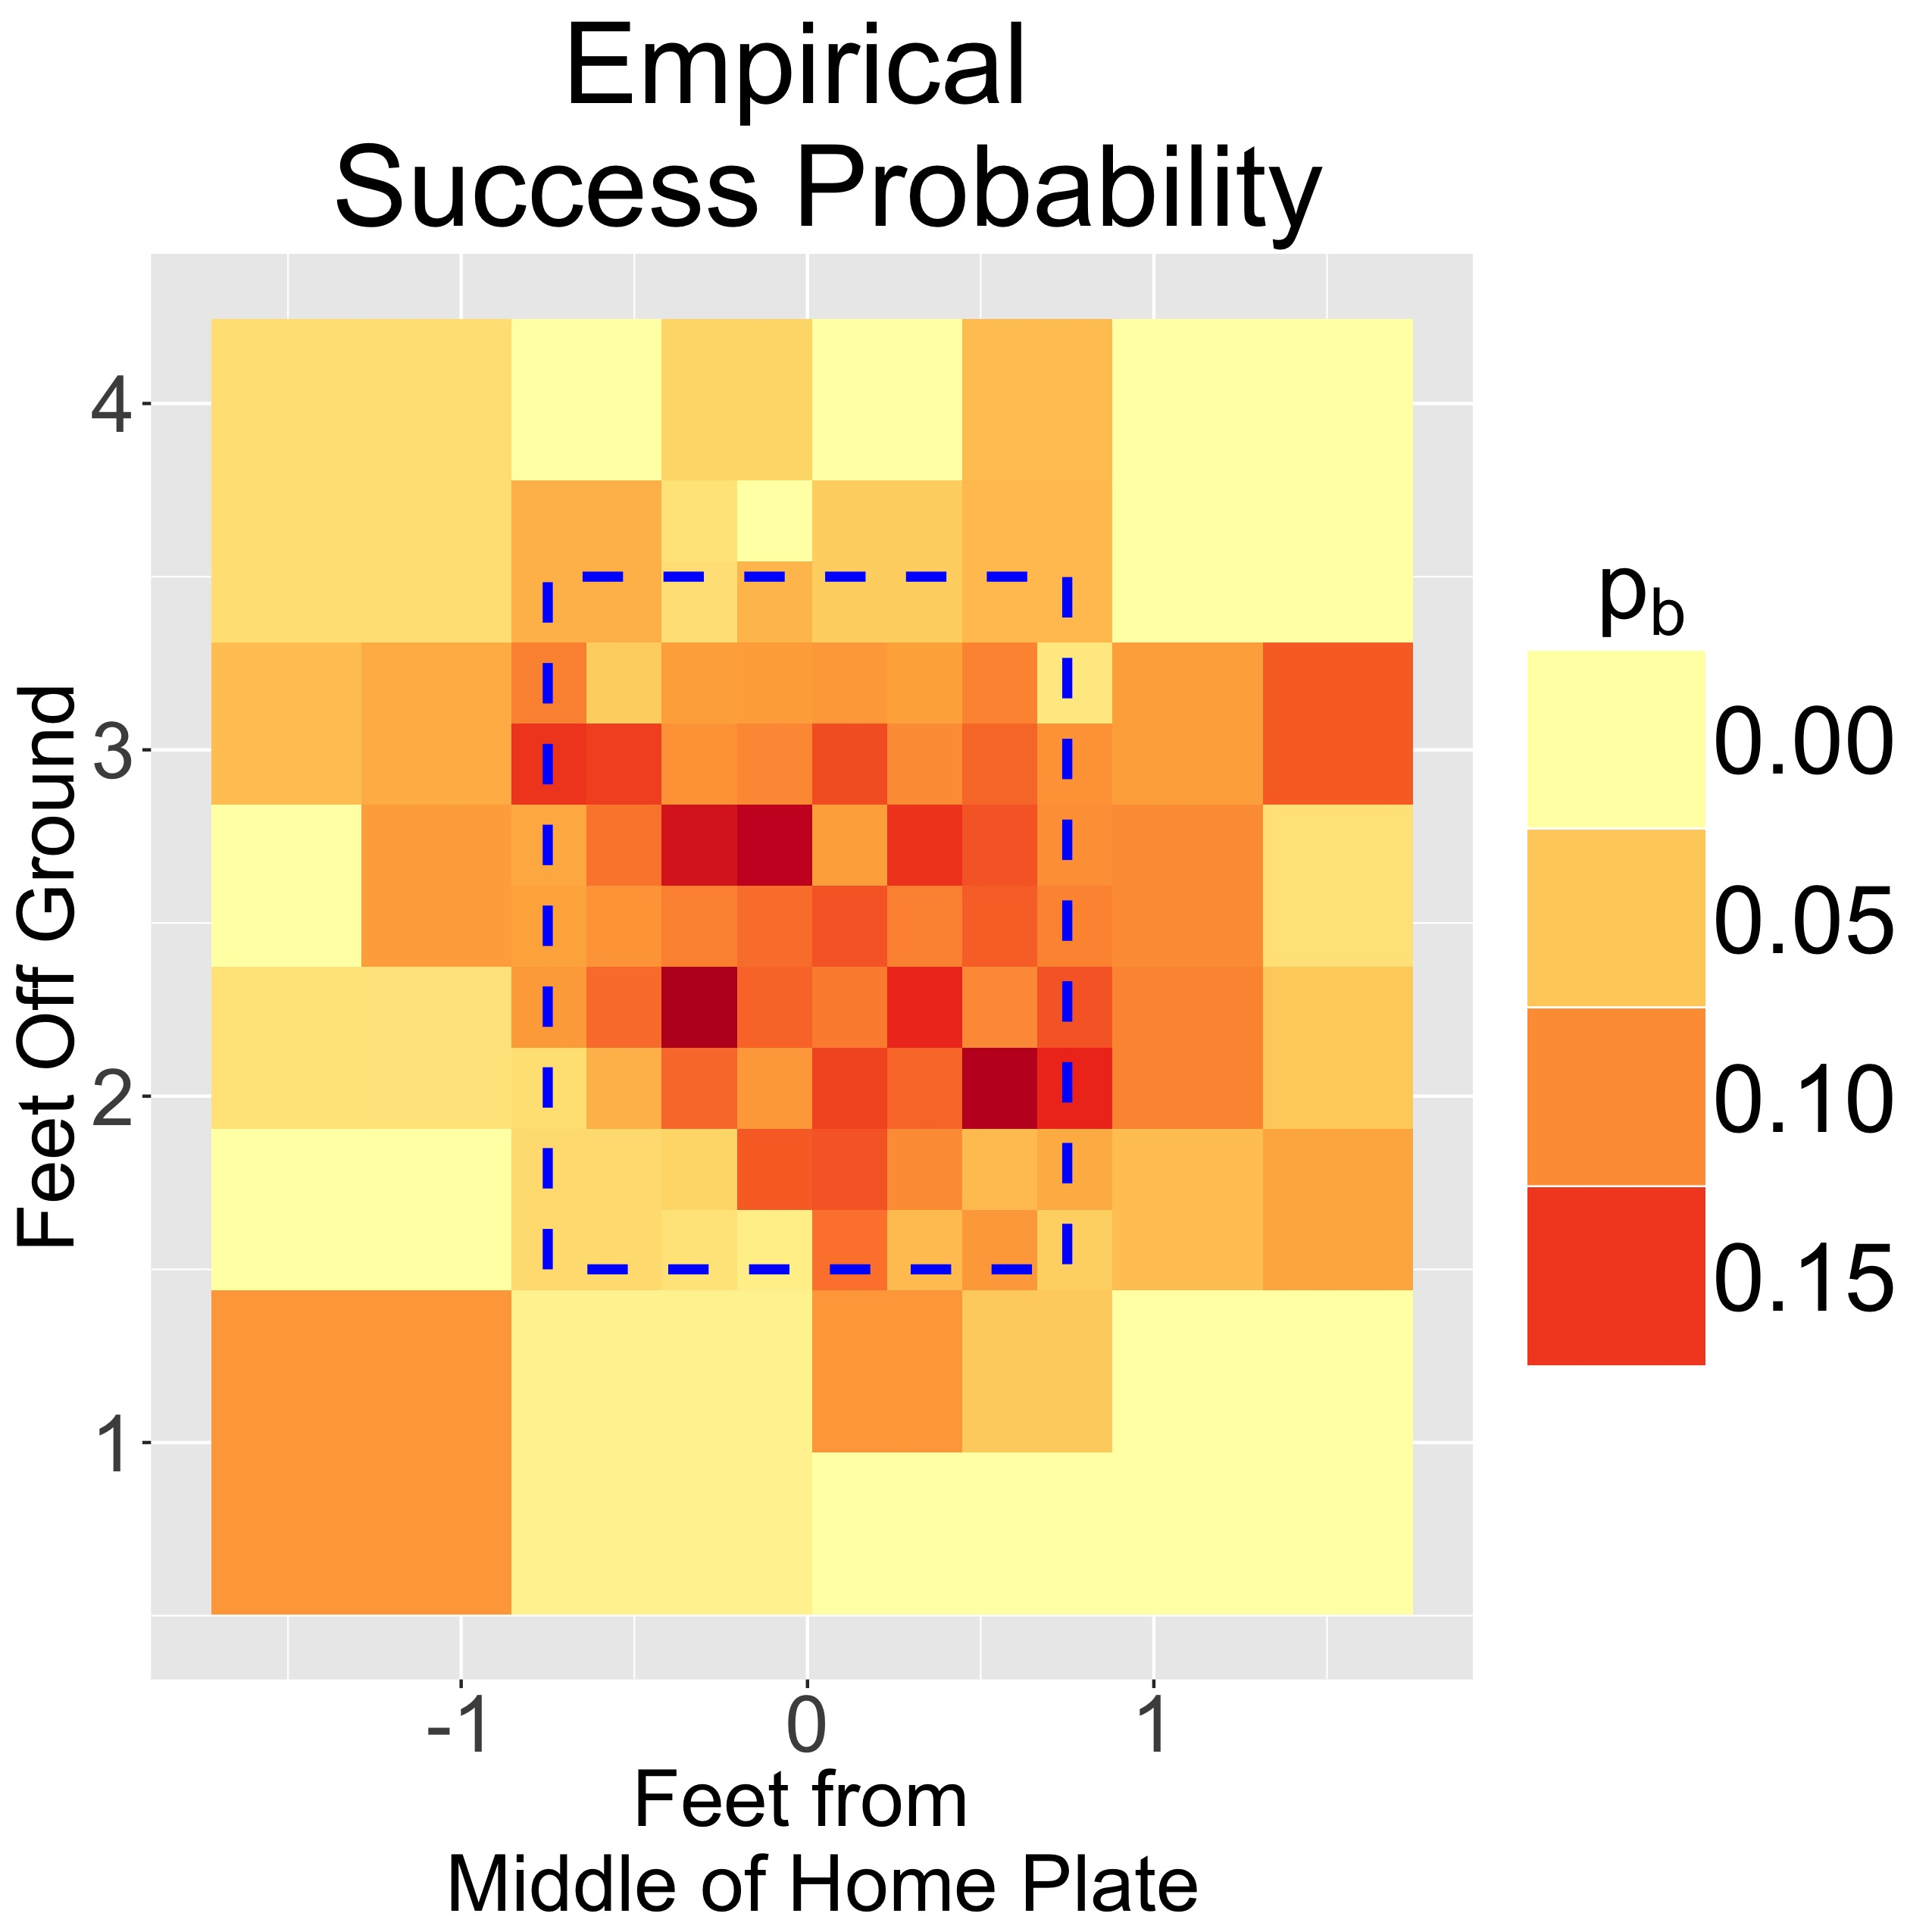
\includegraphics[scale=.06]{Images/Peralta_var-res2.jpg}
% 	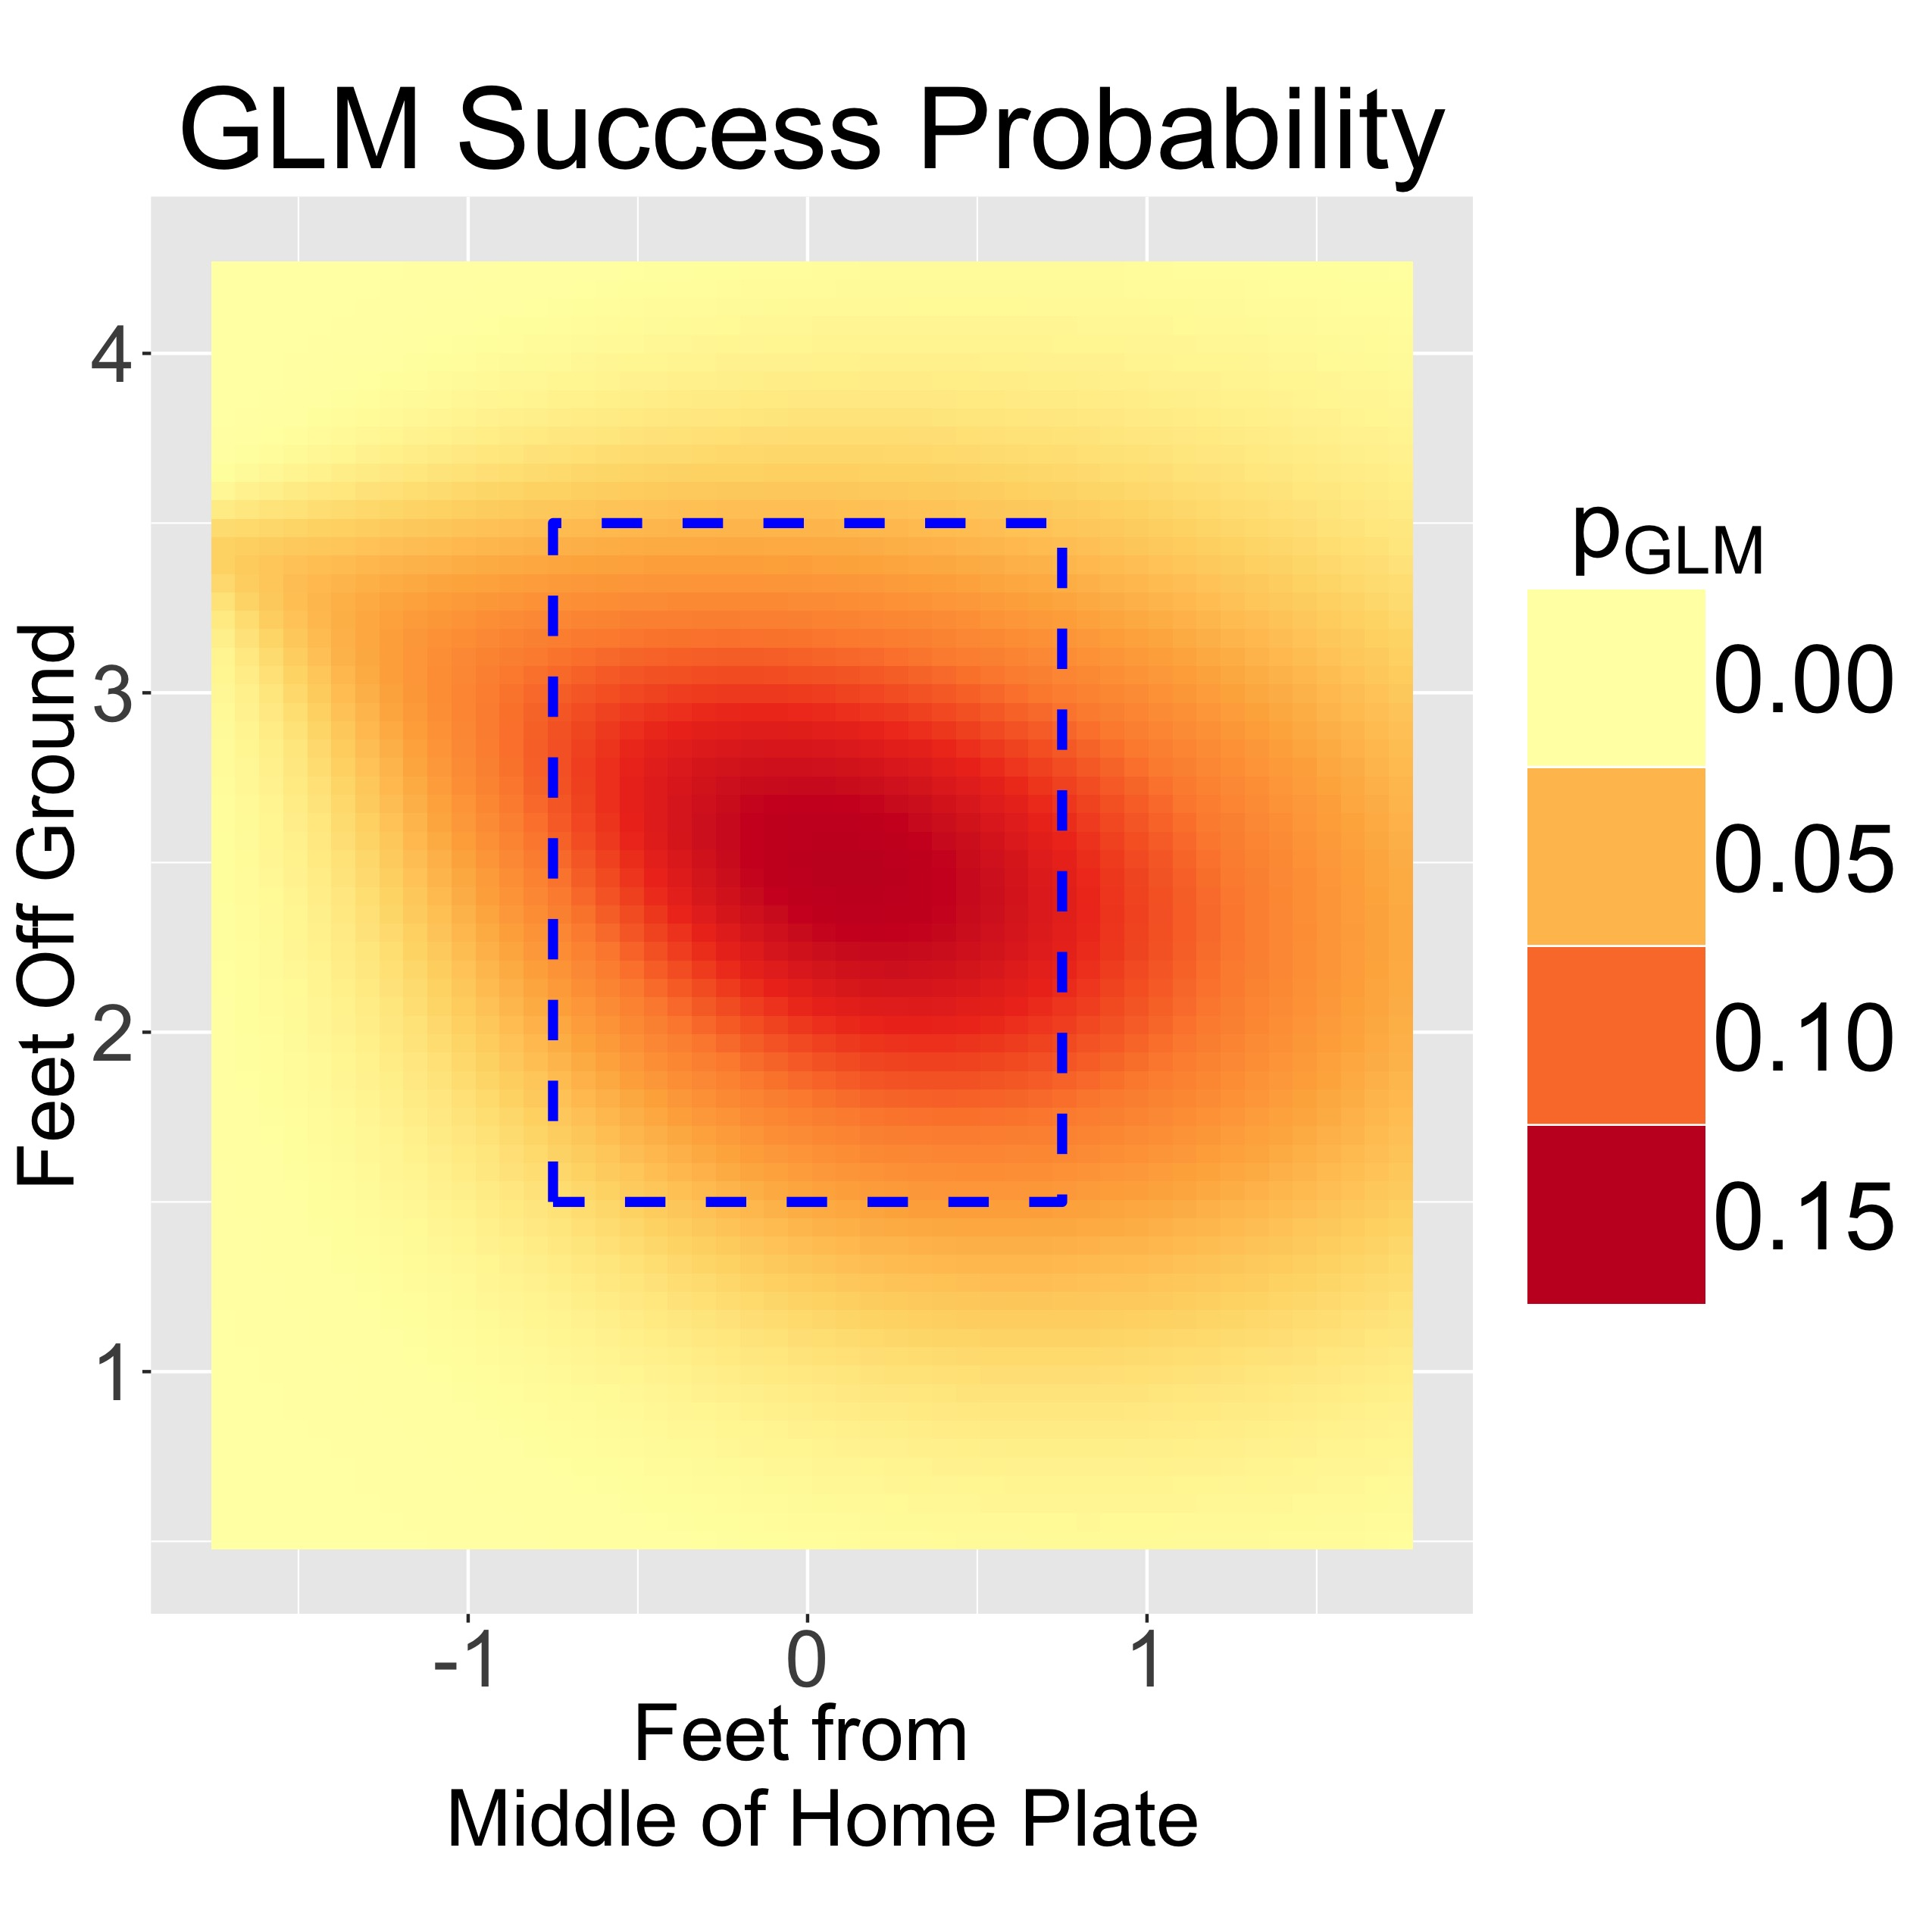
\includegraphics[scale=.06]{Images/Peralta_fit.jpg}
% 	\end{figure}
% 
% \end{frame}
% 
% \begin{frame}{Logistic Regression Model, Jhonny Peralta} % ======
%   \begin{figure}[H]
% 	\centering
% 	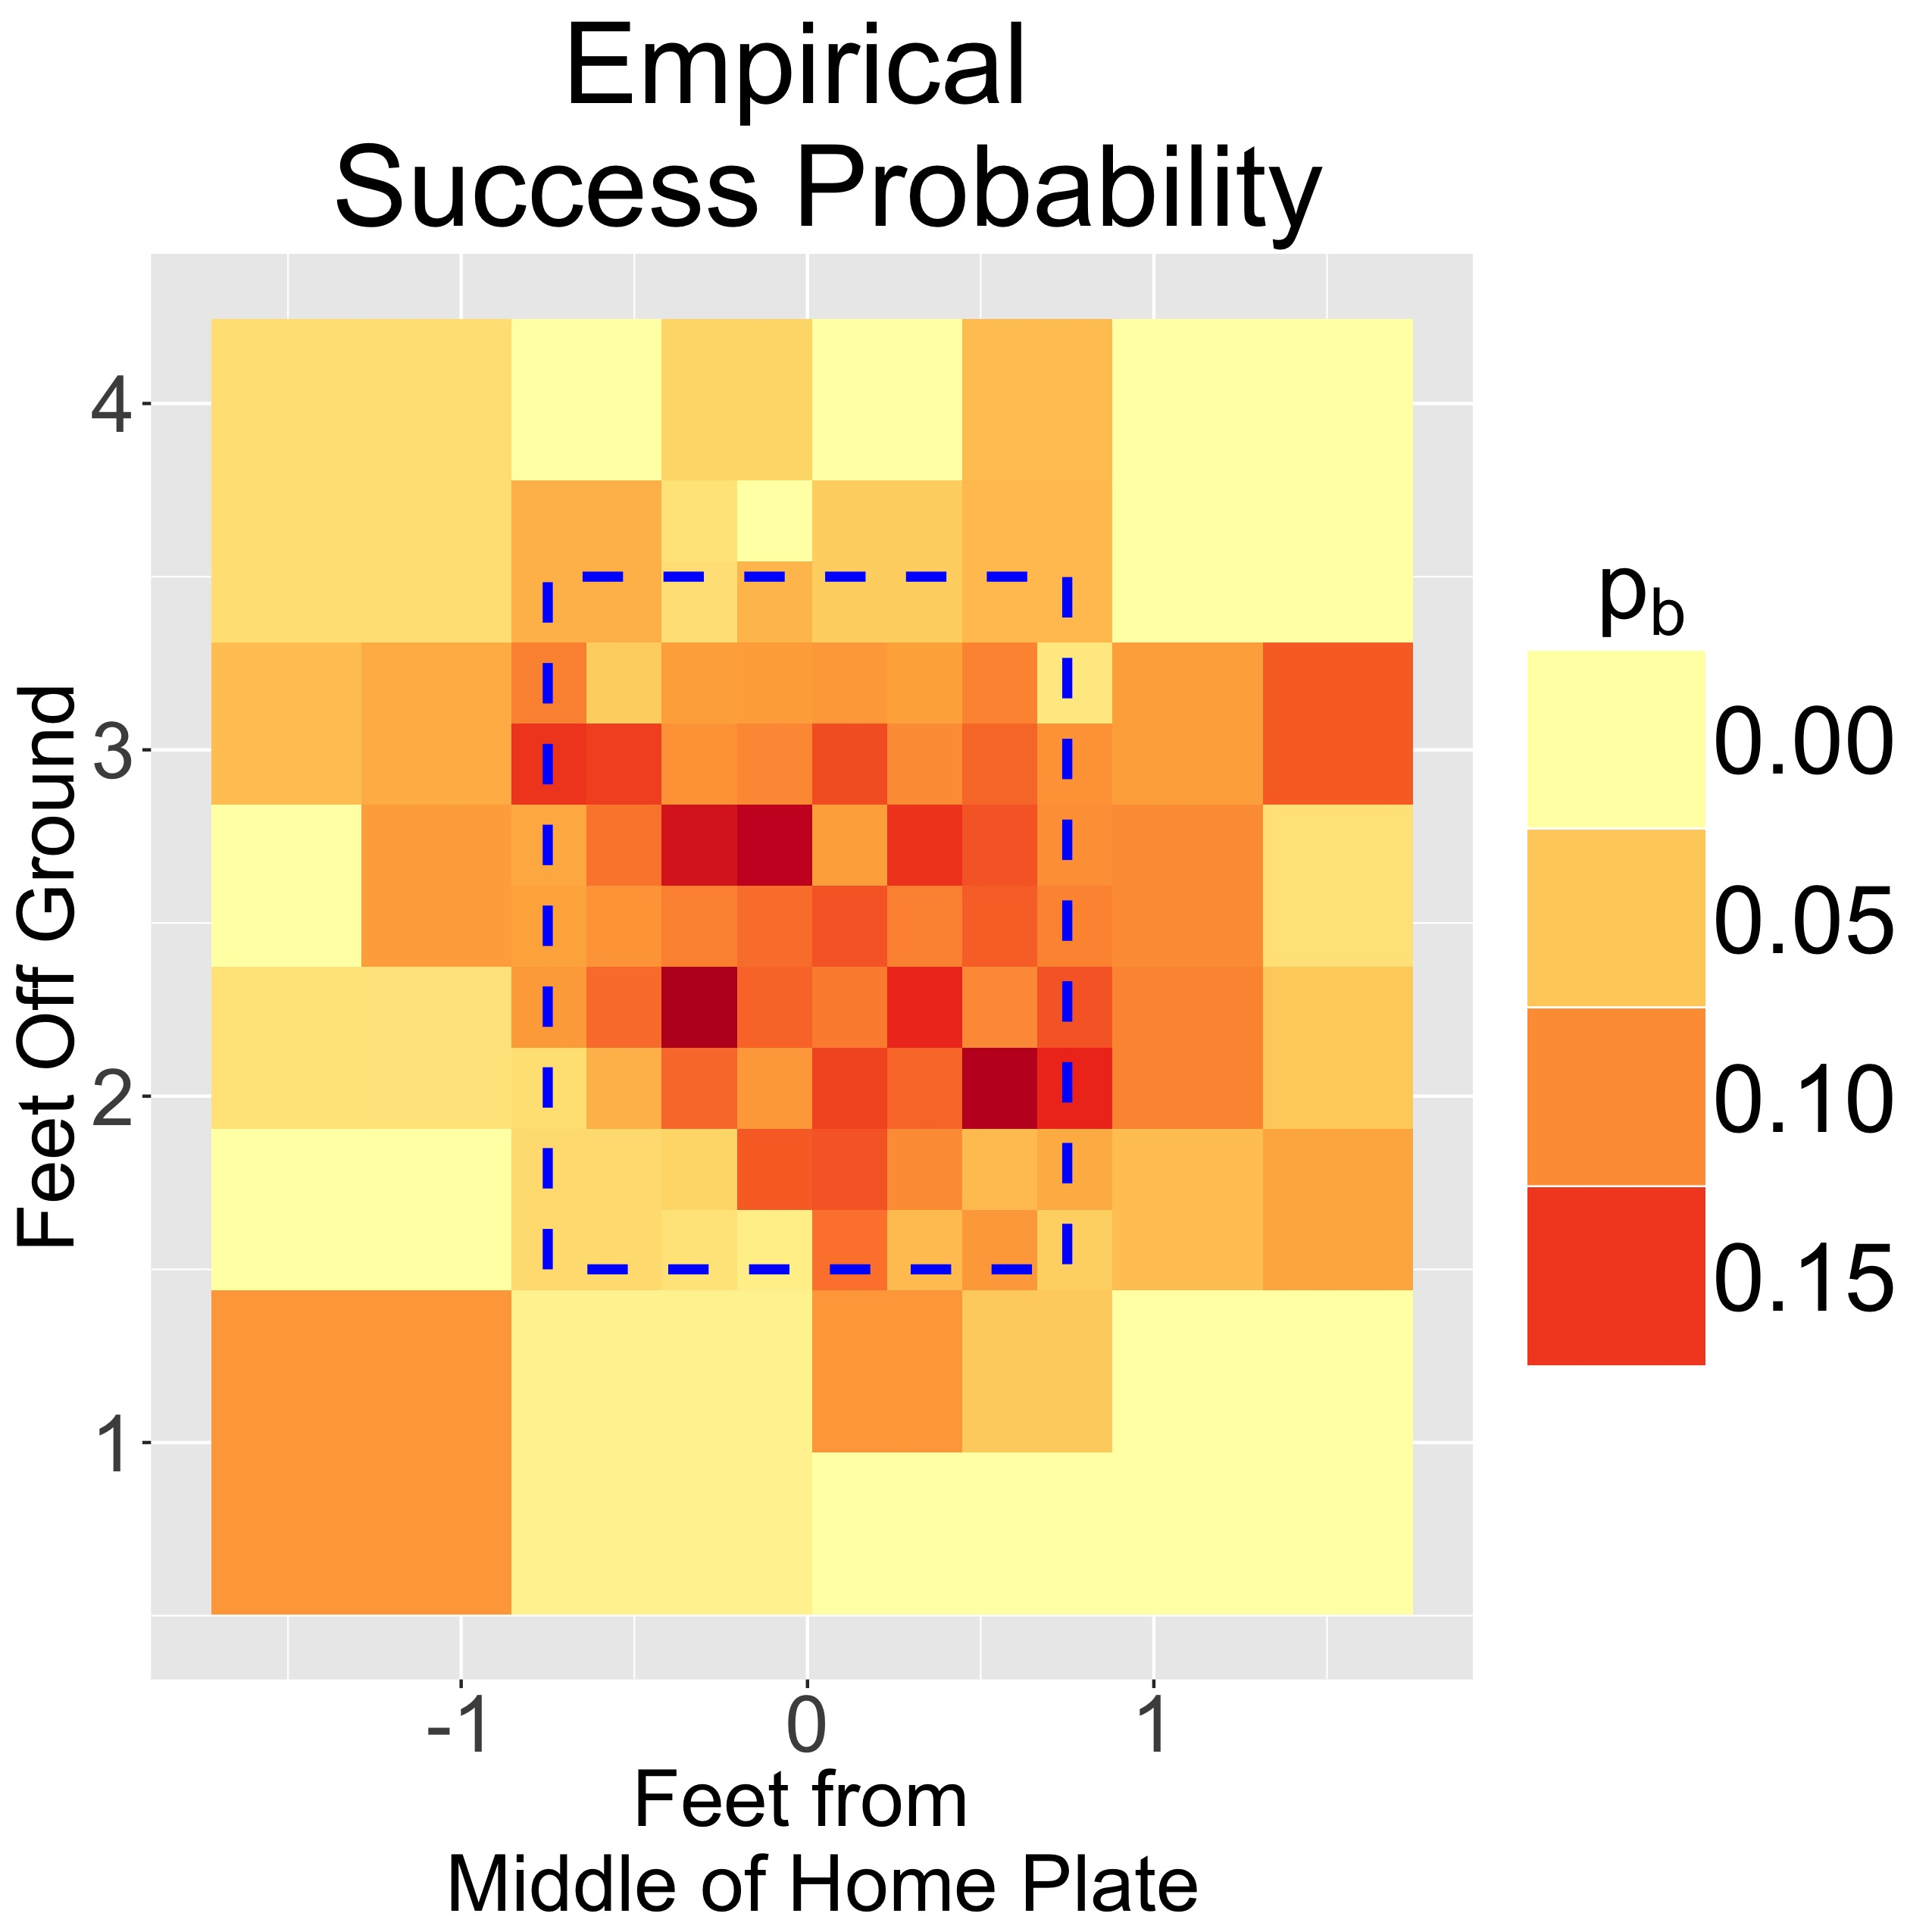
\includegraphics[scale=.05]{Images/Peralta_var-res2.jpg}
% 	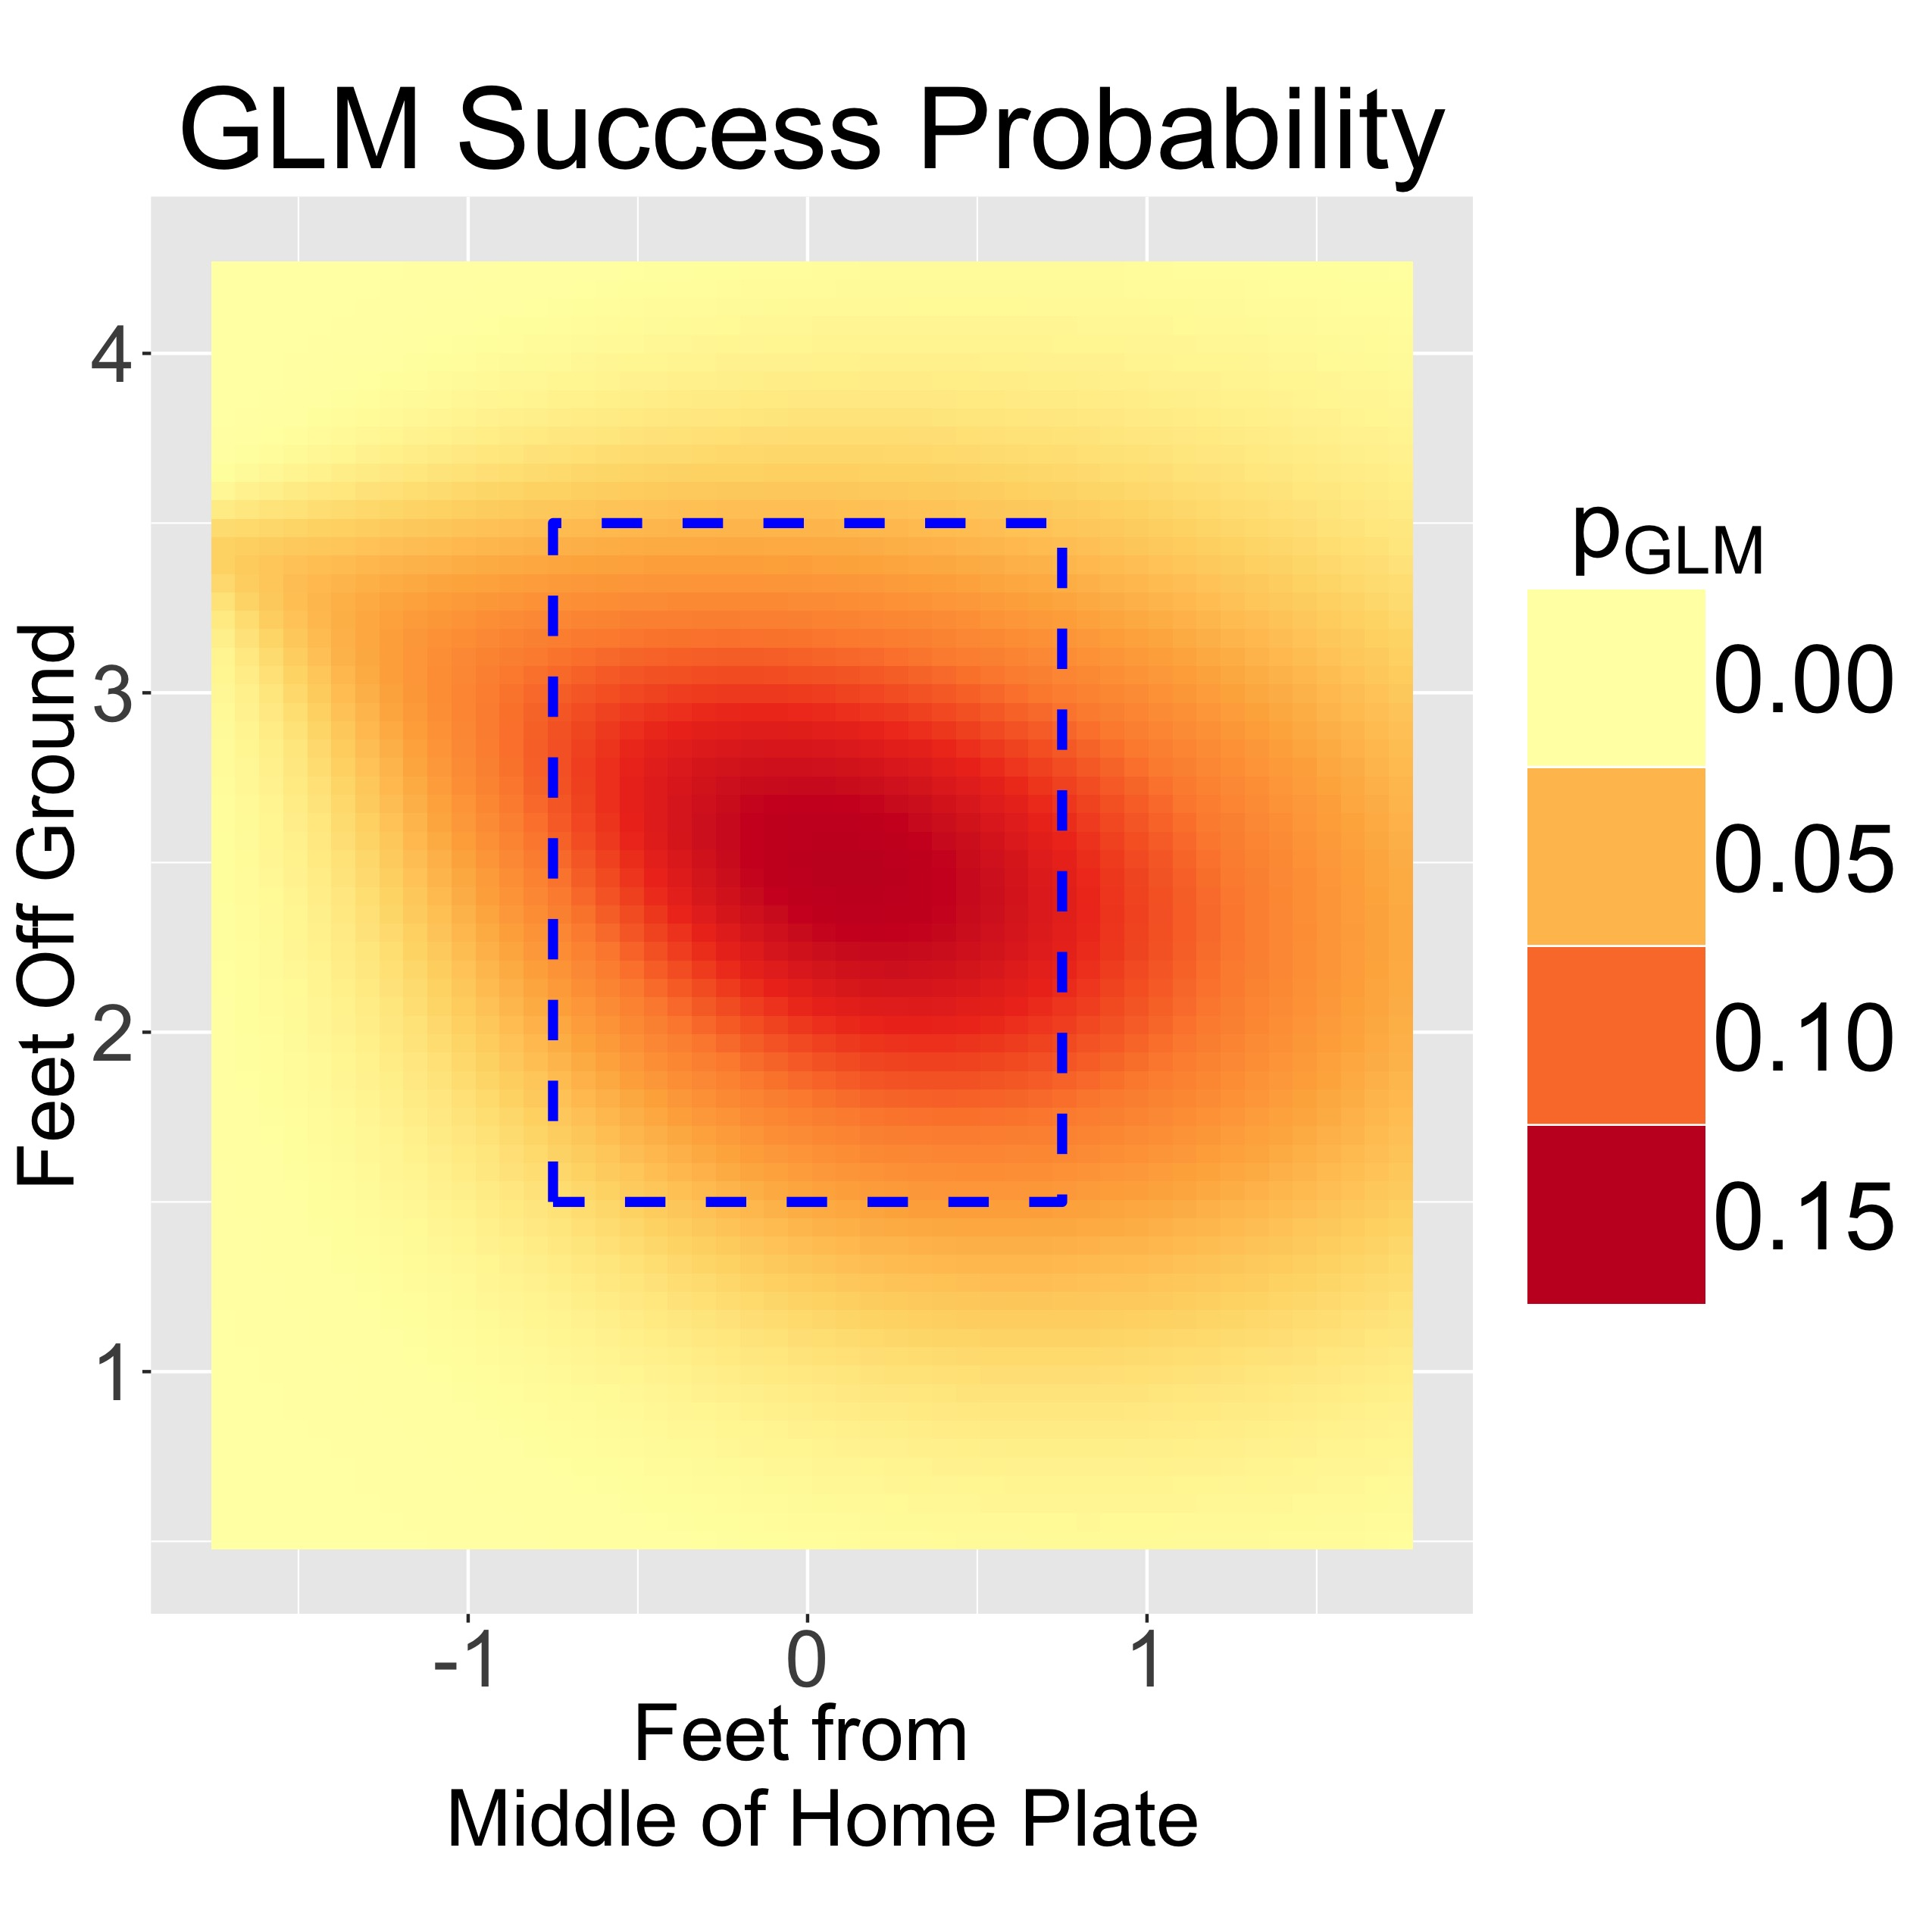
\includegraphics[scale=.05]{Images/Peralta_fit.jpg}
% 	\end{figure}
% \begin{itemize}
% \addtolength{\itemsep}{0.5\baselineskip}
% \item Hosmer-Lemeshow (logistic regression) GOF test
%   \begin{itemize}
%   \addtolength{\itemsep}{0.5\baselineskip}
%   \item Like Pearson $\chi^{2}$ test, but cont. covariates (no categories)
%   \item $H_0$: Well fit \\ $H_A$: Lack of fit
%   \item p-value = 0.8217
%   \end{itemize}
% \end{itemize}
% \end{frame}
% 
% \begin{frame}{Interactive Confidence Intervals}{} % ======
%   \begin{figure}[H]
% 	\centering
% 	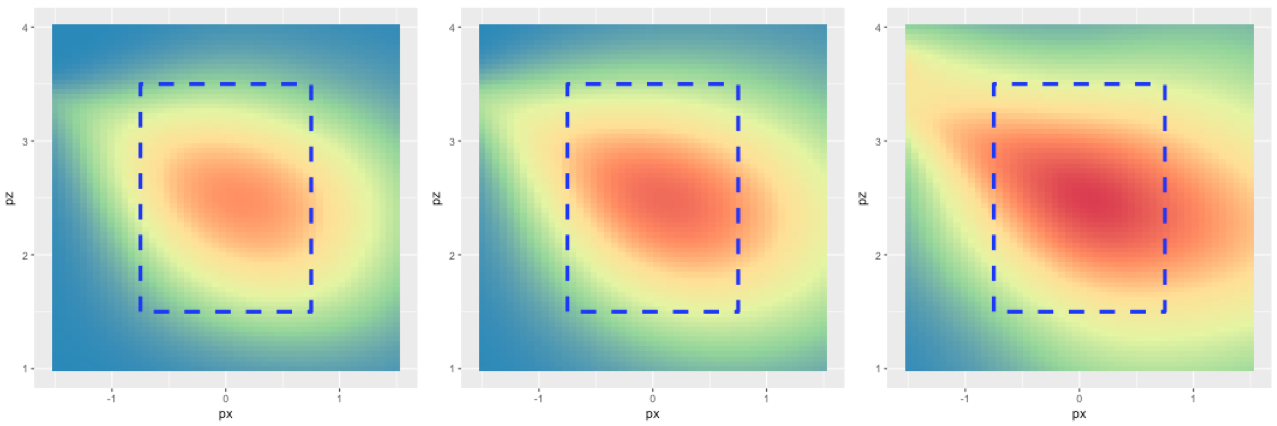
\includegraphics[scale=.275]{Images/99.png}
% 	\end{figure}
% {\bf mapapp}: An R Package
% \end{frame}
% 
% \section{Approaches to Big Data SGLMMs for Baseball Data}
% 
% \begin{frame}{GLM + Spatial Random Effect}{}
% For swings $i = 1, 2, \dots, N$:
% $$ Y_{i}|\mathbf{X}_{i}(\mathbf{s}_{i}) \stackrel{ind}{\sim} \mbox{Bernoulli}(\pi_{i}) $$
% $$\text{logit}(\pi_{i}|\pmb{s}_{i}) = \mathbf{X}_{i}(\mathbf{s}_{i})\beta + w(\pmb{s}_{i}) $$
% \begin{itemize}
% \addtolength{\itemsep}{0.5\baselineskip}
% \item $w(\pmb{s}_{i})$ - spatial random effect at location $\pmb{s}_{i}$.
% \item $\pmb{w}(\pmb{s}) = (w(\pmb{s}_{1}), w(\pmb{s}_{2}), \dots, w(\pmb{s}_{N}))$  - vector of spatial random effects
% \item Tobler's First Law of Geography
% \item Unexplained {\bf spatial} variation in the mean
% \end{itemize}
% \center{$\rightarrow$ Spatial Generalized Linear Mixed Model (SGLMM)}
% \end{frame}
% 
% \begin{frame}{Gaussian Random Field: \pmb{w}(\pmb{s})}{} % ======
% 
% $$\text{logit}(\pi_{i}|\pmb{s}_{i}) = \mathbf{X}_{i}(\mathbf{s}_{i})\beta + w(\pmb{s}_{i}) $$
% \begin{itemize}
% \addtolength{\itemsep}{0.5\baselineskip}
% \item Gaussian Random Field (GRF) \\
%   \begin{itemize}
%   \item $\pmb{w}(\pmb{s}) | \pmb{\theta} \sim MVN(\pmb{0}, \Sigma(\pmb{\theta}))$
%   \end{itemize}
% \item Exponential covariance
% $$ \Sigma(\phi, \sigma^{2})_{i,k} = \text{Cov}(w(\pmb{s}_{i}), w(\pmb{s}_{k})) =  \sigma^{2} \text{exp}(-||\pmb{s}_{i} - \pmb{s}_{k}||/\phi)$$
%   \begin{itemize}
%   \addtolength{\itemsep}{0.5\baselineskip}
%   \item $||s_{i} - s_{k}||$ - Euclidean distance between $\pmb{s}_{i}$ and $\pmb{s}_{k}$
%   \item $\sigma^{2}$ - scale parameter
%   \item $\phi$ - range parameter.
%   \end{itemize}
% \end{itemize}
% \end{frame}
% 
% 
% \begin{frame}{``Big N'' Problem}
% \begin{itemize}
% \addtolength{\itemsep}{0.5\baselineskip}
% \item Computational cost increases at a rate of $\mathcal{O}(n^{3})$: 
% $$t(n) \leq M \cdot n^{3} \text{ as } n \rightarrow \infty$$
% \item Recall: iterative MCMC approach, invert high dimension matrices
% \item GRF $\pmb{w}$, with $n \times n$ correlation matrix
% \item Every iteration requires $\Sigma^{-1}$, determinant of $\Sigma$
% \end{itemize}
% \end{frame}
% 
% \subsection{Computational Optimization in Stan}
% 
% \begin{frame}{Hamiltonian Markov Chain (HMC) in Stan}
% \begin{itemize}
% \addtolength{\itemsep}{0.5\baselineskip}
% \item Proposal distribution - key component of MCMC algorithm
% \item Stan proposal machinery: HMC, from physics (molecular motion)
%   \begin{itemize}
%   \addtolength{\itemsep}{0.5\baselineskip}
%   \item $H(q(t),p(t)) = U(q(t)) + K(p(t))$
%   \item Total energy of a system
%   \item t = time
%   \item {\bf q = position (variables of interest)}, U = potential energy
%   \item p = momentum (auxiliary), K = kinetic energy
%   \end{itemize}
% \item $H(q,p) = -\text{log}f_{q}(q) + p^{T}\pmb{M}^{-1}p/2$
% \item Tidy partial derivatives
% \item {\bf Short version}: randomly sample momentum p (auxiliary), calculate new position q  --- that's your Metropolis proposal.
% \end{itemize}
% \end{frame}
% 
% 
% \begin{frame}[fragile]{Stan Optimization}{}
% \begin{itemize}
% \addtolength{\itemsep}{0.5\baselineskip}
% \item Informative (sharp tailed) prior on exponential covariance length-scale parameter $\phi$ for model identifiability (normal or log-normal)
% \item Computing time/convergence - ``Complex models'' such as spatial hierarchical models require proper priors for all $\pmb{\beta}$ coefficients.
% \item QR factorization on covariate matrix X; reparameterize, adjust priors
% \begin{align*}
% \pmb{X} &= \pmb{QR} \\
% \pmb{X \beta} &= \pmb{QR \beta} \rightarrow \text{Let } \pmb{\theta} = \pmb{R \beta} \\
% \pmb{X \beta} &= \pmb{Q \theta} \\
% \pmb{\beta} &= \pmb{R^{-1}\theta}
% \end{align*}
% \end{itemize}
% \end{frame}
% 
% \begin{frame}[fragile]{Stan Optimization}{}
% \begin{itemize}
% \addtolength{\itemsep}{0.5\baselineskip}
% \item Add noise to the covariance matrix diagonal, ensure numerical positive-definiteness
% \item Cholesky decomposition and tactical reparameterization
%     \begin{verbatim}
%     L = cholesky_decompose(Sigma);
%     Z ~ normal(0, 1);
%     Z_mod = L * Z;
%     Y ~ bernoulli_logit(Q*theta + Z_mod);
%     \end{verbatim}
% \item Matrix algebra and vectors, over ‘for loops’ and scalars
% \begin{verbatim}
% hit ~ bernoulli_logit(X*beta + Z)
% \end{verbatim}
% is faster than
% \begin{verbatim}
% for (n in 1:N)
%     hit[n] = bernoulli_logit(X[n]*beta[n] + Z[n]);
% \end{verbatim}
% \end{itemize}
% \end{frame}
% 
% 
% \begin{frame}{Stan Model Fitting} % ===== ====== ===== ===== =====
% \begin{itemize}
% \addtolength{\itemsep}{0.5\baselineskip}
% \item N = 1000: 7 hours 45 mins for 1500 draws
%   \begin{itemize}
%   \item Note: w/o spatial effect: 6 seconds.
%   \end{itemize}
% \item N = 2000 overnight, 350 draws
% \end{itemize}
%   \begin{figure}[H]
% 	\centering
% 	\includegraphics[scale=.32]{Images/Turtle.png}
% 	\end{figure}
% \end{frame}

% \begin{frame}{PPM Procedure}{Nuts and Bolts} % ===== ====== ===== ===== =====
% \begin{align*}
% \text{logit}(\pi_{i}|\pmb{s}_{i}) &= \pmb{X}_{i}(\pmb{s}_{i}) \pmb{\beta} + w(\pmb{s}_{i}) \\
% \pmb{w}(\pmb{s}) | \pmb{\theta} &\sim \text{GRF}(\pmb{0}, \pmb{\Sigma}(\pmb{\theta}))
% \end{align*}
% \begin{itemize}
% \addtolength{\itemsep}{0.5\baselineskip}
% \item $\pmb{w}(\pmb{s})$ - $n \times 1$ vector of random effects, at locations $\pmb{s}$
% \item $\pmb{0}$ - $n \times 1$ zero vector
% \item $\Sigma(\pmb{\theta})$ - $n \times n$, symmetric, positive-definite covariance matrix
%     \begin{itemize}
%     \item $\pmb{\theta}$ - covariance parameters
%     \end{itemize}
% \item $\Sigma(\pmb{s}_{i}, \pmb{s}_{k}; \pmb{\theta})$ - covariance of random effects at locations $\pmb{s}_{i}$ and $\pmb{s}_{k}$
%       \begin{itemize}
%       \addtolength{\itemsep}{0.5\baselineskip}
%       \item $\Sigma(\pmb{\theta}) = [\Sigma(\pmb{s}_{i}, \pmb{s}_{k}; \pmb{\theta})]_{i,k=1}^{n}$
%       \end{itemize}
% \end{itemize}
% \end{frame}
% 
% \begin{frame}{PPM Knots} % ===== ====== ===== ===== =====
% \begin{itemize}
% \addtolength{\itemsep}{0.5\baselineskip}
% \item $\pmb{S}^{*} = \{\pmb{s}_{1}^{*}, \dots, \pmb{s}_{m}^{*}\}$ --- $m$ knot locations
%   \begin{itemize}
%   \item $m < < n$
%   \end{itemize}
% \item $\pmb{w}^{*} = \left[w(\pmb{s}_{i}^{*})\right]_{i=1}^{m}$ -- knot location random effects
% \item $\pmb{w}^{*}|\pmb{\theta} \sim \text{GRF}\{\pmb{0}, \Sigma^{*}(\pmb{\theta})\}$ -- $m$-dimensional GRF \\
% \item $\Sigma^{*}(\pmb{\theta}) = \left[\Sigma(\pmb{s}_{i}^{*}, \pmb{s}_{k}^{*})\right]_{i,k = 1}^{m}$ -- $m \times m$ knot covariance matrix
% \end{itemize}
% \end{frame}
% 
% \begin{frame}{PPM, Kriging} % ===== ====== ===== ===== =====
% \begin{itemize}
% \addtolength{\itemsep}{0.5\baselineskip}
% \item $\pmb{\sigma}(\pmb{s}_{0};\pmb{\theta}) = \left[\Sigma(\pmb{s}_{0}, \pmb{s}_{k}^{*}; \pmb{\theta})\right]_{k = 1}^{m}$ --- $m \times 1$ vector, $\text{Cov}(w(\pmb{s}_{0}), \text{ knots})$
% \item  $\widetilde{w}(\pmb{s}_{0})$ - interpolated random effect
%         \begin{align*}
%         \widetilde{w}(\pmb{s}_{0}) &= E[w(\pmb{s}_{0})|\pmb{w}^{*}] \\
%         &= \pmb{\sigma}^{T}(\pmb{s}_{0};\pmb{\theta}) \cdot \Sigma^{*-1}(\pmb{\theta}) \cdot \pmb{w}^{*}
%         \end{align*}
% \item Spatially varying linear combination
% \item Minimizes squared error loss function (linear predictors, GRFs)
% \end{itemize}
% 
% Now replace $w(\pmb{s}_{i})$ with $\widetilde{w}(\pmb{s}_{i})$.
% \end{frame}
% 
% \begin{frame}[fragile]{The Predictive Process: $\widetilde{w}(\pmb{s})$}
% Another Gaussian Random Field
% \begin{align*}
% \widetilde{\pmb{w}}(\pmb{s}) &\sim \text{GRF}\{0, \widetilde{\Sigma}(\cdot)\} \\
% \widetilde{\Sigma}(\pmb{s}, \pmb{s}'; \pmb{\theta}) &= \pmb{\sigma}^{T}(\pmb{s};\pmb{\theta}) \cdot \textcolor{blue}{\pmb{\Sigma}^{*-1}(\pmb{\theta})} \cdot \pmb{\sigma}(\pmb{s}';\pmb{\theta})
% \end{align*}
% Predictive process model:
%     \begin{equation}
%     \text{logit}(\pi_{i}|\pmb{s}_{i}) = \pmb{X}_{i}(\pmb{s}_{i}) \pmb{\beta} + \widetilde{w}(\pmb{s}_{i}) \nonumber
%     \end{equation}
%     \begin{itemize}
%     \item Note dimension of \textcolor{blue}{covariance matrix}.
%     \item Implement in \verb|spBayes| \citep{Finley2013}.
%     \item Faster?
%     \end{itemize}
% \end{frame}
% 
% \begin{frame}{PPM ``Results''}
% 
% \textcolor{red}{*No convergence.*}
% 
%       \begin{itemize}
%       \addtolength{\itemsep}{0.5\baselineskip}
%       \item n = 500, knots = 97, 10K samples, $\approx$ 4 mins
%       \item n = 1000, knots = 97, 10K samples, $\approx$ 6.7 mins
%       \item n = 1000, knots = 49, 30K samples, $\approx$ 7 mins
%       \item n = 3000, knots = 49, 80K samples, $\approx$ 54 mins
%       \end{itemize}
% \end{frame}

\section{Integrated Nested Laplace Approximation (INLA)}

\begin{frame}{INLA Overview}
$$ \text{logit}(\pi_{i}) = \pmb{X}_{i}(\pmb{s}_{i})\pmb{\beta} + w(\pmb{s}_{i}) $$
\begin{itemize}
\addtolength{\itemsep}{0.5\baselineskip}
\item Approximation for Bayesian hierarchical models with latent GRF
\item Essentially a two part process for continuous domain
  \begin{itemize}
  \addtolength{\itemsep}{0.5\baselineskip}
  \item Part 1: Represent Mat\'ern GRF as GMRF (SPDE)
  \item Part 2: Numerically integrate posterior approximation (INLA)
  \end{itemize}
\end{itemize}
  \begin{figure}[H]
	\centering
	\includegraphics[scale=.02]{Images/BL.jpg}
	\end{figure}
\end{frame}

\begin{frame}{Part 1: Mat\'ern GRF as GMRF \citep{Lindgren2011}}

\begin{itemize}
\addtolength{\itemsep}{0.5\baselineskip}
% \item Use Mat\'ern covariance structure for GRF $\pmb{w}(\pmb{s})$
% \item Goal: represent GRF $\pmb{w}(\pmb{s})$ as GMRF $\widetilde{\pmb{w}}(\pmb{s})$ 
%   \begin{itemize}
%   \addtolength{\itemsep}{0.5\baselineskip}
%   \item Sparse precision matrix
%   \end{itemize}
\item Finite Element Method: project SPDE onto basis representation
\item Stochastic partial differential equation (SPDE)
$$ (\kappa^{2} - \Delta)\pmb{w}(\pmb{s}) = \pmb{W}(\pmb{s})$$
\item Piecewise linear basis representation
$$ \widetilde{w}(\pmb{s}) = \sum_{k} \psi_{k}(\pmb{s})\omega_{k}$$
        \begin{itemize}
        \addtolength{\itemsep}{0.5\baselineskip}
        \item Triangulation of domain
        \item $\psi_{k}(\pmb{s})$ --- deterministic basis functions
        \item $\omega_{k}$ --- weights, explicit and sparse precision matrix
        \end{itemize}
\end{itemize}

\end{frame}

\begin{frame}{Part 1: Mat\'ern GRF as GMRF \citep{Lindgren2011}}{(Continued)}

\begin{itemize}
\addtolength{\itemsep}{0.5\baselineskip}
\item Definition: $\langle f(\pmb{u}), g(\pmb{u}) \rangle = \int f(\pmb{u}) g(\pmb{u}) d\pmb{u}$

\item Basis representation and SPDE:
$$ \widetilde{w}(\pmb{s}) = \sum_{k} \psi_{k}(\pmb{s})\omega_{k} \longrightarrow (\kappa^{2} - \Delta)\widetilde{\pmb{w}}(\pmb{s}) = \pmb{W}(\pmb{s})  $$
\item Galerkin solution:
$$ \left(
\kappa^{2} \pmb{C} + \pmb{G} \right) \pmb{\omega} \overset{D}{=} \text{N}(\pmb{0},\pmb{C})$$
Where $\pmb{C} = \langle \psi_{l}, \psi_{k} \rangle$, and $ \pmb{G} = \langle \psi_{l}, - \Delta \psi_{k} \rangle$
\item $\pmb{\omega} \sim \text{N}(\pmb{0}, \pmb{Q}^{-1})$ for 
$$\pmb{Q} = \left( \kappa^{2} \widetilde{\pmb{C}} + \pmb{G} \right)^{T} \pmb{C}^{-1} \left( \kappa^{2} \widetilde{\pmb{C}} + \pmb{G} \right).$$
\end{itemize}

\end{frame}

\begin{frame}{Part 2, Integrated Nested Laplace Approximation (INLA) \citep{Rue2009}}

\begin{itemize}
\addtolength{\itemsep}{0.5\baselineskip}
\item Parameter vector: $\pmb{\rho} = ( \pmb{\beta}^{\text{T}}, \widetilde{\pmb{w}}^{\text{T}} )^{\text{T}}$
            \begin{itemize}
            \addtolength{\itemsep}{0.5\baselineskip}
            \item Let $\pmb{Q}$ denote the precision matrix of $\pmb{\rho}$
            \end{itemize}
\item Hyperparameter vector: $\pmb{\theta} = \{\kappa, \sigma \}$
\end{itemize}
INLA Steps
\begin{itemize}
\item Gaussian approximation:
$$ p_{G}(\pmb{\rho}|\pmb{\theta}, \pmb{y}) \propto \text{exp} \left( -\frac{1}{2}(\pmb{\rho-\mu})^{T} (\pmb{Q} + \text{diag}(\pmb{c}) ) (\pmb{\rho - \mu}) \right) $$
              \begin{itemize}
              \item $\pmb{c}$ and $\pmb{\mu}$ depend on second order Taylor expansions of $f(\pmb{\rho}) = \sum_{i} \text{log }p(y_{i}|\pmb{\rho},\pmb{\theta})$
              \end{itemize}
\end{itemize}
\end{frame}


\begin{frame}{Part 2, INLA \citep{Rue2009}}{Continued}
\begin{itemize}
\addtolength{\itemsep}{0.5\baselineskip}
\item For a given $\pmb{\theta}$, let $\pmb{\rho}_{0} = \text{argmax}_{\rho}p(\pmb{\rho}|\pmb{y},\pmb{\theta})$. Then,
$$  p(\pmb{\theta}|\pmb{y}) \approx \tilde{p}(\pmb{\theta}|\pmb{y}) \propto  \frac{p(\pmb{y} | \pmb{\rho}_{0}, \pmb{\theta}) p(\pmb{\rho}_{0} | \pmb{\theta})}{p_{G}(\pmb{\rho}_{0} | \pmb{y}, \pmb{\theta})} \cdot p(\pmb{\theta}) $$
$\longrightarrow \hat{\pmb{\theta}}_{\text{ML}} \approx \text{argmax}_{\theta} \tilde{p}(\pmb{\theta}|\pmb{y})$
\item Numerical integration: 
        $$ p(\rho_{j} | \pmb{y}) \approx \int p_{\text{G}}(\rho_{j}|\pmb{\theta, y})\tilde{p}(\pmb{\theta}|\pmb{y}) d\pmb{\theta} $$
\item Numerical integration: 
$$ p(\theta_{k} | \pmb{y}) \approx \int \tilde{p}(\pmb{\theta}|\pmb{y}) d\pmb{\theta}_{-k} $$
\end{itemize}

\end{frame}

\begin{frame}{3000 Words}{Variable-resolution, GLM, SGLMM with INLA}
  \begin{figure}[H]
	\centering 	
	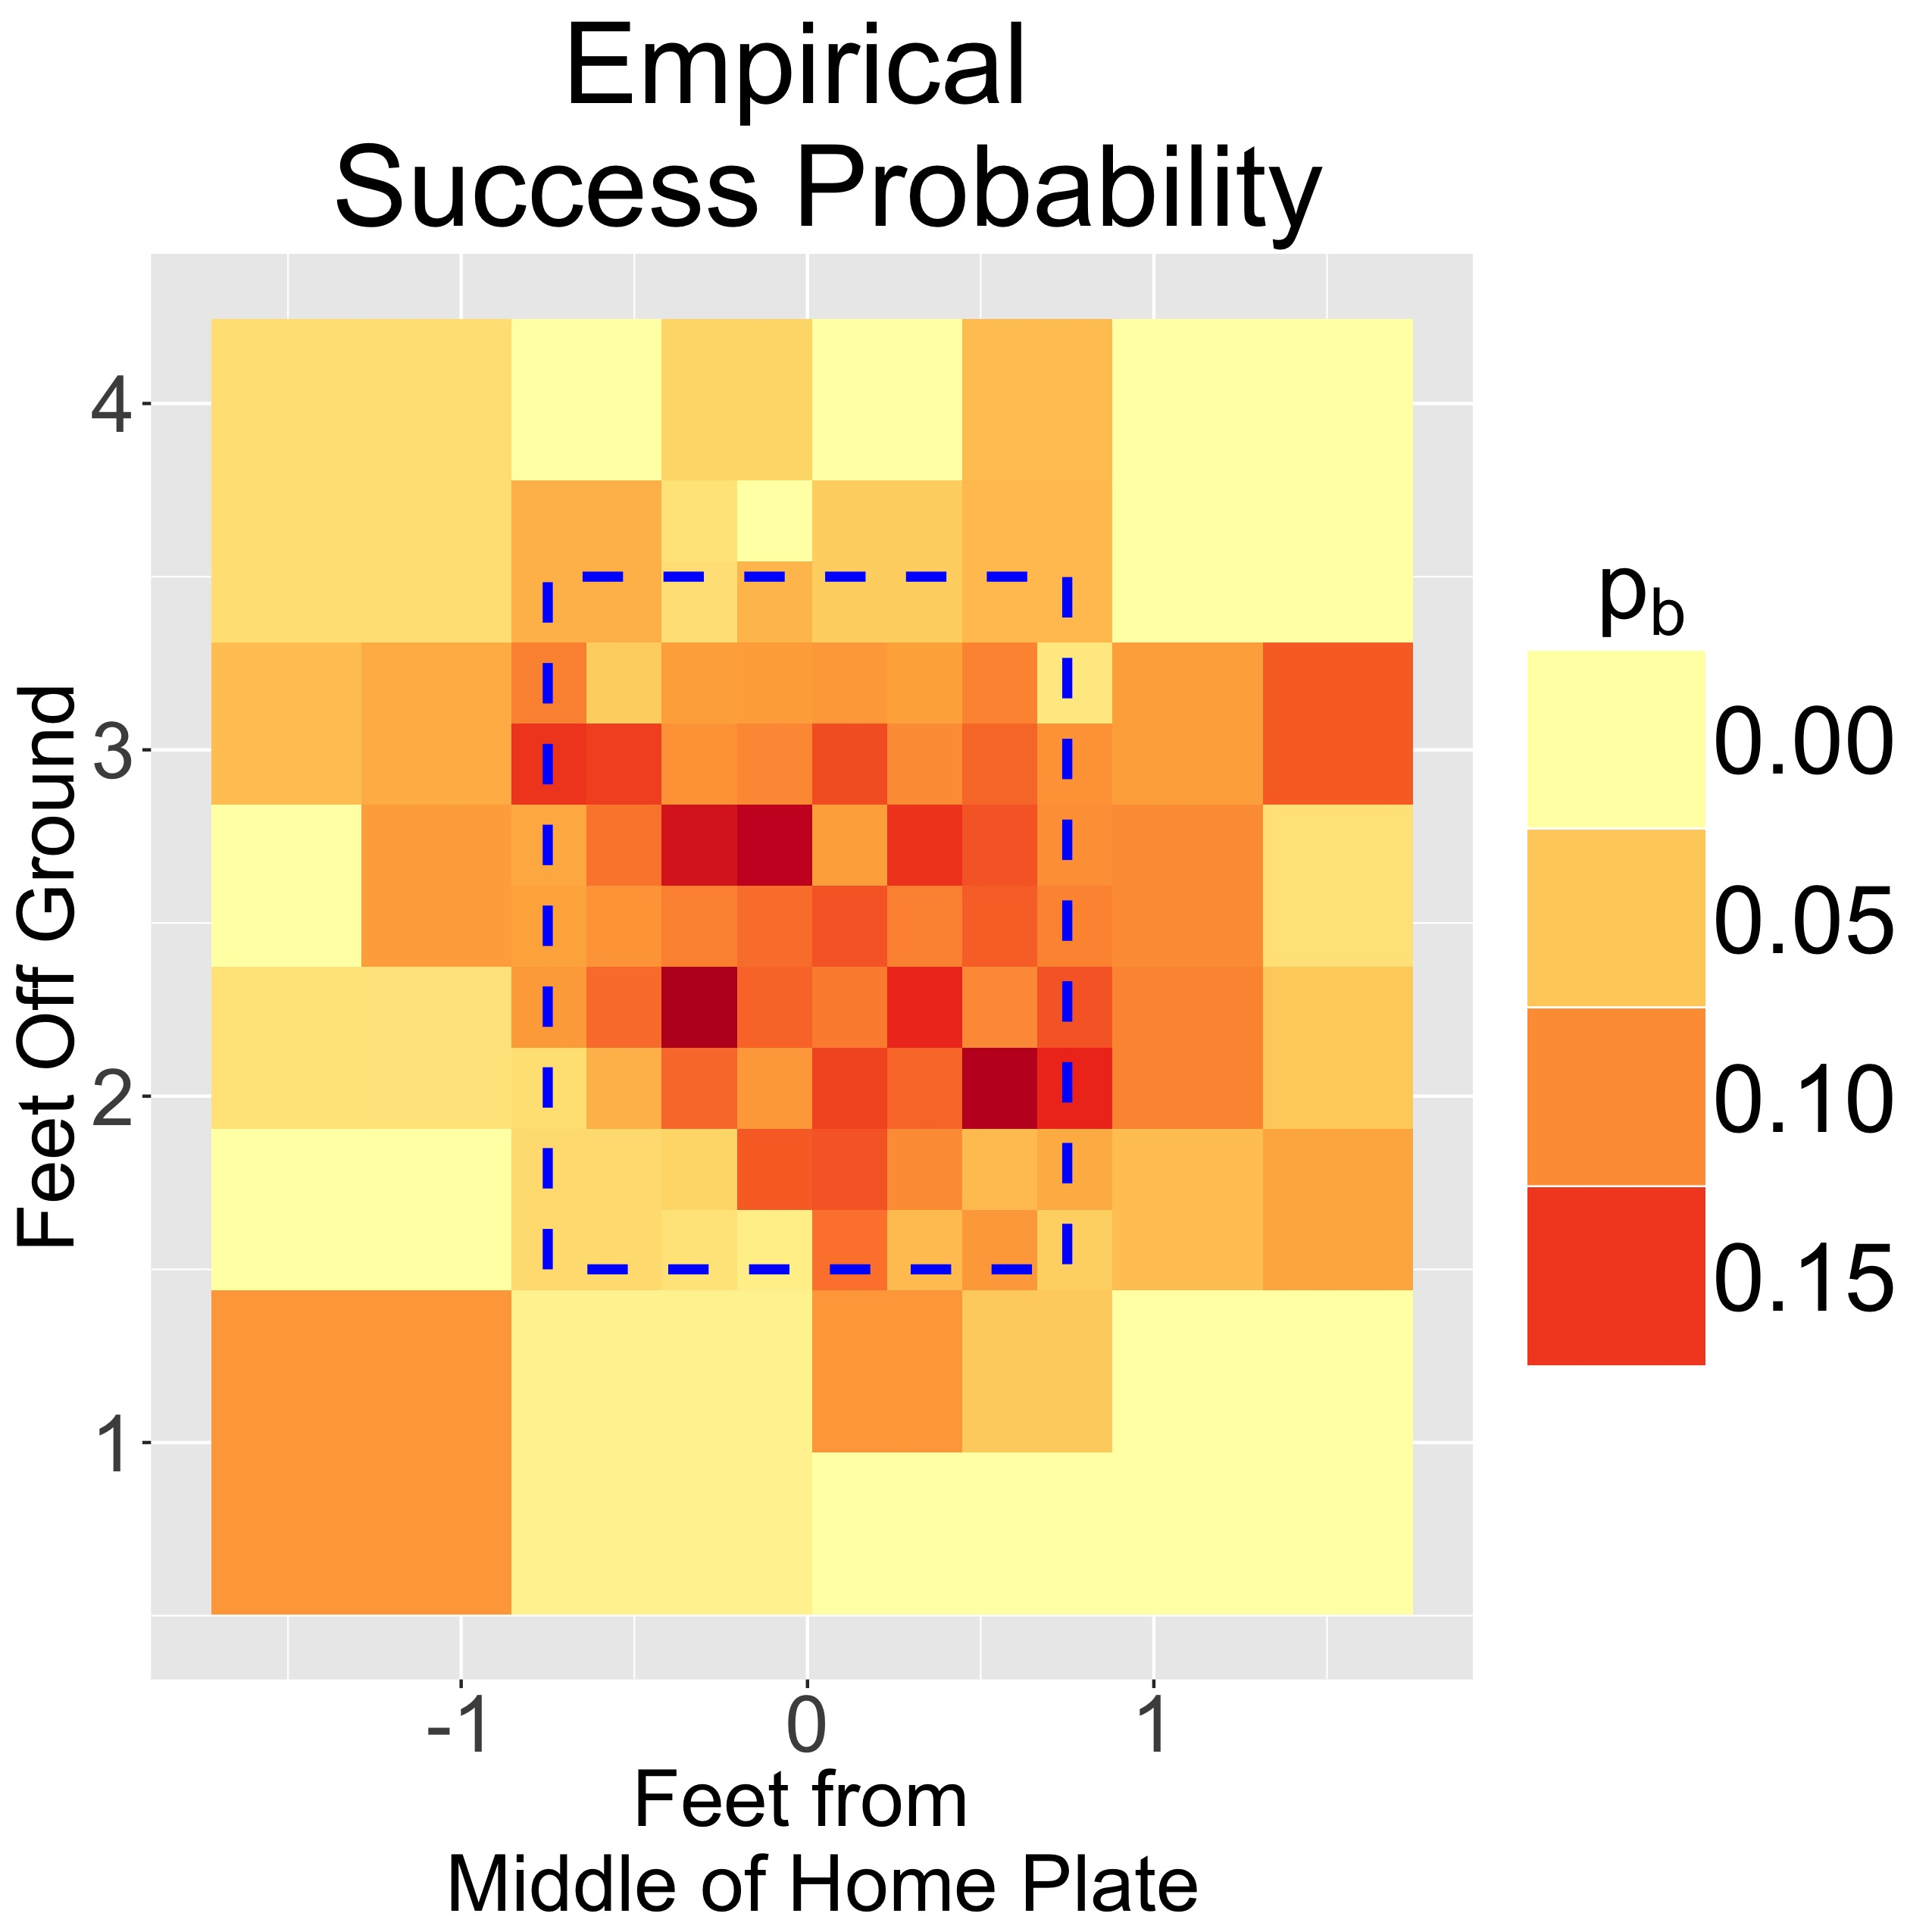
\includegraphics[scale=.04]{Images/Peralta_var-res2.jpg}
	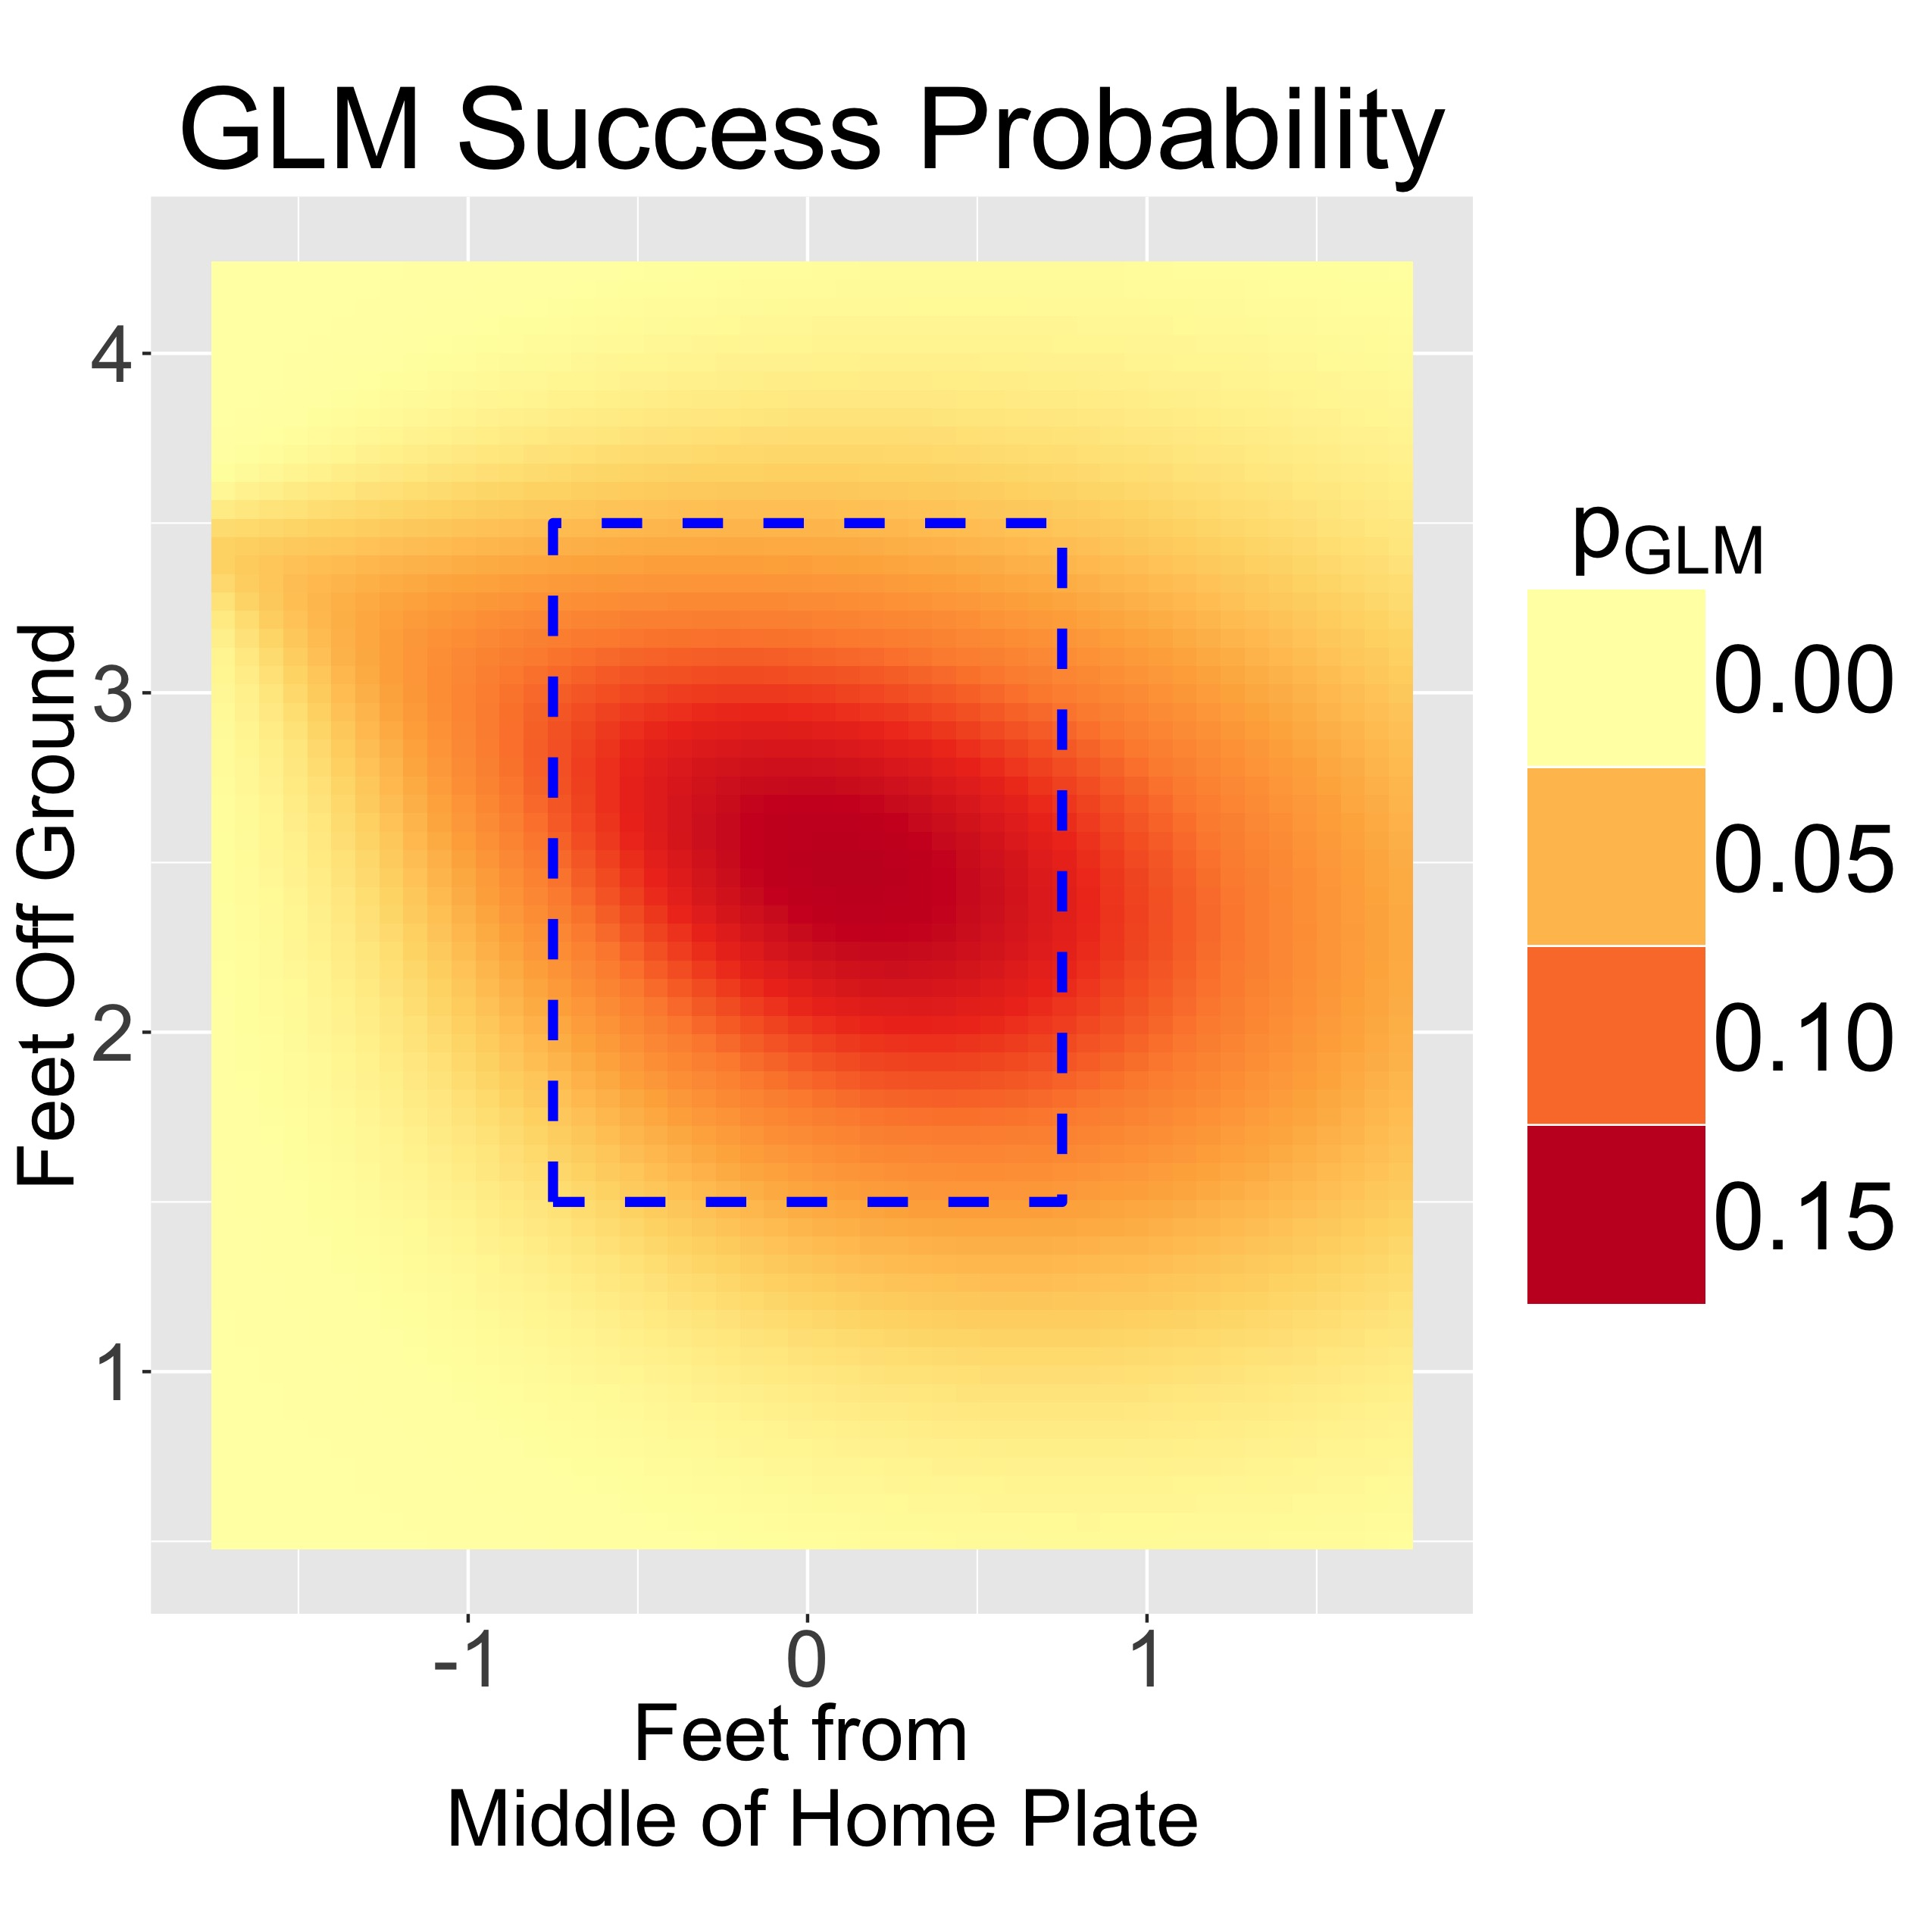
\includegraphics[scale=.04]{Images/Peralta_fit.jpg}
	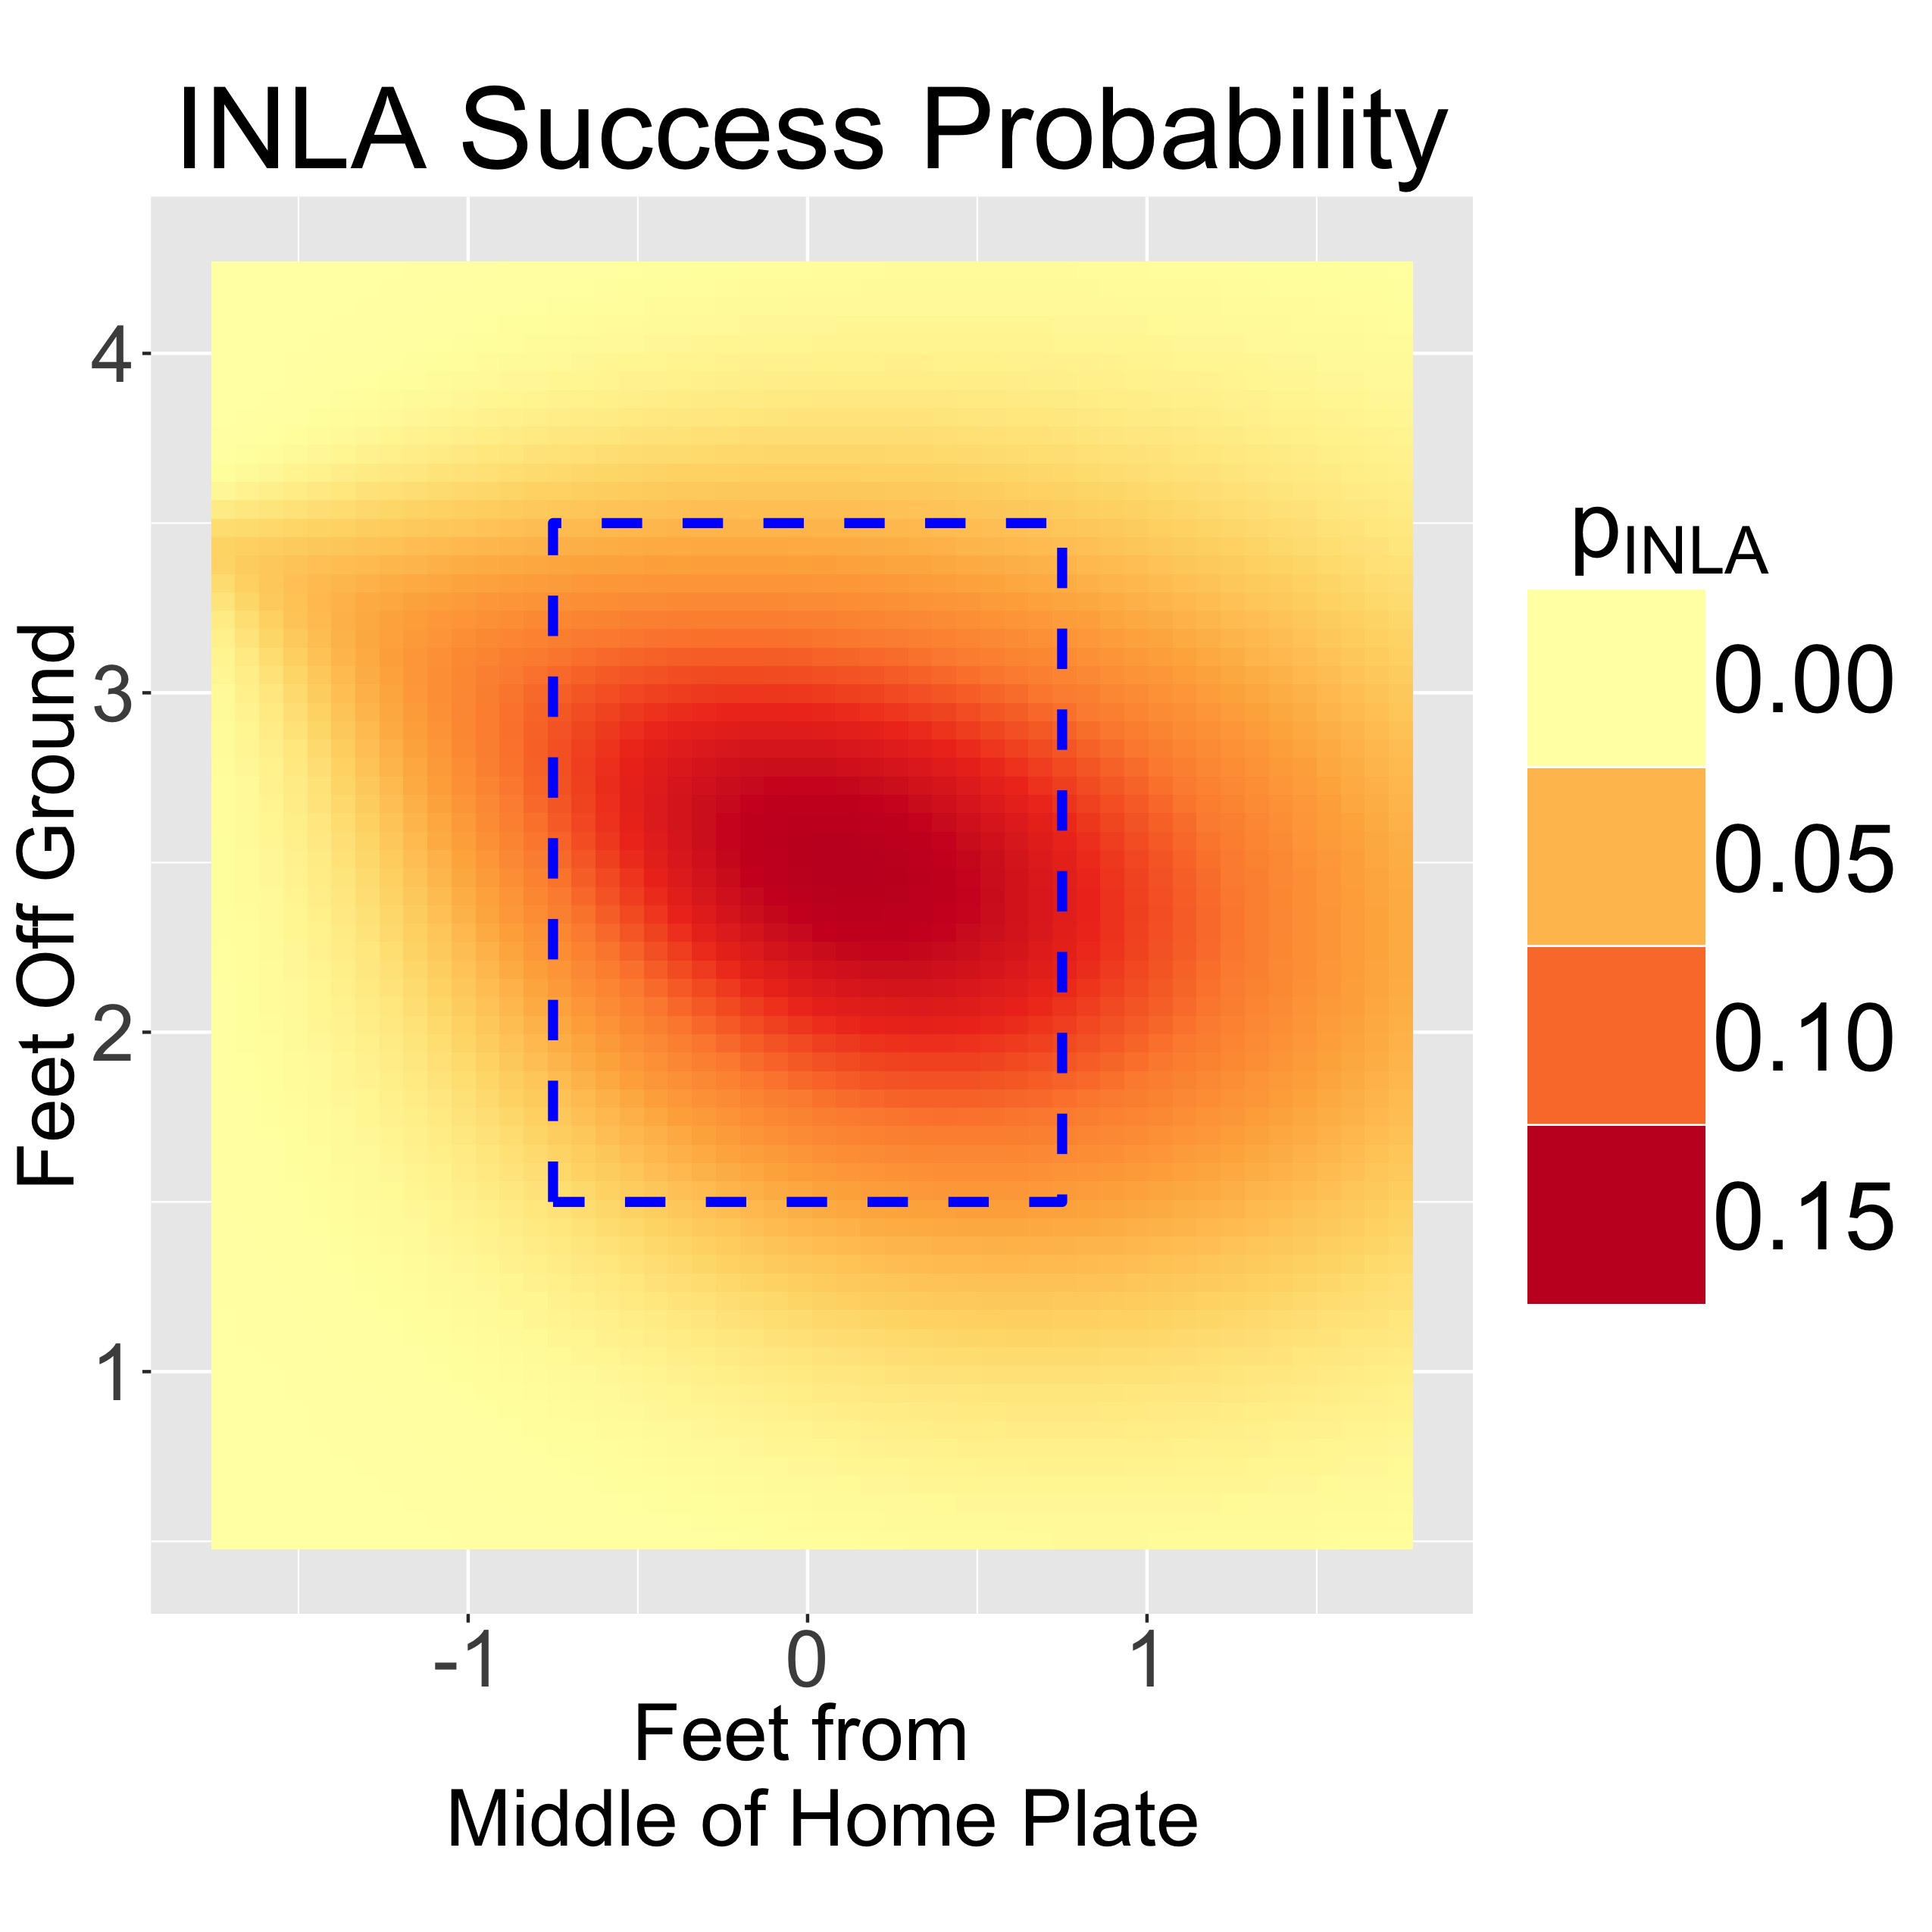
\includegraphics[scale=.04]{Images/INLA.jpg}
	\end{figure}
\end{frame}

\begin{frame}{Estimates}


\begin{table}
\scalebox{0.85}{
\begin{tabular}{| l | c | c | c |}
\hline
\multicolumn{4}{|c|}{} \\
\multicolumn{4}{|c|}{} \\
\multicolumn{4}{|c|}{GLM} \\
\hline
Covariate         & $\beta_{i}$ & MLE   & SE   \\ \hline
1                 & $\beta_{0}$ & -4.08 & 0.70 \\ \hline
r                 & $\beta_{1}$ &  1.19 & 0.51 \\ \hline
$\theta$          & $\beta_{2}$ & -1.93 & 1.90 \\ \hline
$r*\theta$        & $\beta_{3}$ & -1.64 & 0.70 \\ \hline
$r^{2}$           & $\beta_{4}$ & -0.32 & 0.09 \\ \hline
$\theta^{2}$      & $\beta_{5}$ & -3.92 & 1.10 \\ \hline
$r^{2}*\theta^{2}$& $\beta_{6}$ & -0.46 & 0.21 \\ \hline
\end{tabular}
\quad
\begin{tabular}{| l | c | c | c |}
\hline
\multicolumn{4}{|c|}{INLA} \\
\hline
Covariate         & $\rho _{i}$ & $\hat{\rho}_{i}$ & SE \\ \hline
N/A               & $\kappa$    &  3.23 & $\pm$ 1 SE: (1.35, 7.54) \\ \hline
N/A               & $\sigma$    &  0.11 & $\pm$ 1 SE: (0.05, 0.26) \\ \hline
1                 & $\beta_{0}$ & -4.14 & 0.76 \\ \hline
r                 & $\beta_{1}$ &  1.25 & 0.55 \\ \hline
$\theta$          & $\beta_{2}$ & -1.90 & 1.96 \\ \hline
$r*\theta$        & $\beta_{3}$ & -1.70 & 0.93 \\ \hline
$r^{2}$           & $\beta_{4}$ & -0.33 & 0.10 \\ \hline
$\theta^{2}$      & $\beta_{5}$ & -3.93 & 1.14 \\ \hline
$r^{2}*\theta^{2}$& $\beta_{6}$ & -0.48 & 0.22 \\ \hline
\end{tabular}
}
\end{table}
\begin{itemize}
\item $\hat{\kappa}$ - long range correlation; $\text{SE}(w(\pmb{s})) = 0.11$. 
\item $\rightarrow 0.15 \pm 1 \cdot \text{SE} = (0.137, 0.165)$
\item $\rightarrow 0.15 \pm 2 \cdot \text{SE} = (0.125, 0.181)$
\end{itemize}
\end{frame}

\begin{frame}{Summary}
\begin{itemize}
\item Resolution selection? Variable-resolution heat maps and {\bf varyres}
\item Heat map confidence intervals? Interactive HMCIs and {\bf mapapp}
\item Fitting big data SGLMMs to baseball data?
  \begin{itemize}
  \item Stan - insufficicent
  \item PPM - Slow and did not converge; to be continued...
  \item INLA - Fast, successful; to be continued...
  \end{itemize}
\end{itemize}
\end{frame}


% 
% \begin{itemize}
% \addtolength{\itemsep}{0.5\baselineskip}
% \item Computational costs - increase at a rate of $\mathcal{O}(n^{3/2})$
% \item Trade-offs - speed for bias (Binomial data)
% \end{itemize}
% 
% \begin{frame}{Next Steps}
% \begin{itemize}
% \addtolength{\itemsep}{0.5\baselineskip}
% \item Cool SPDE-INLA pictures
% \item Model evaluation, scoring rules \citep{Bickel2007}
% \item Cross validation study
% \end{itemize}
% \end{frame}
% 
\begin{frame}{}
\begin{center}
\Huge{Thanks for listening.
Questions?}
\end{center}
\end{frame}

\bibliography{Baseball}



\end{document}







